\documentclass[english, 10pt]{article}
\usepackage[sexy]{evan}
\usepackage{inconsolata}
\usepackage[shellescape]{gmp}
\usepackage{titlesec}
\usepackage{color}
\usetikzlibrary{arrows.meta}
\definecolor{editorGray}{rgb}{0.95, 0.95, 0.95}
\definecolor{editorOcher}{rgb}{1, 0.5, 0} % #FF7F00 -> rgb(239, 169, 0)
\definecolor{editorGreen}{rgb}{0, 0.5, 0} % #007C00 -> rgb(0, 124, 0)
\usepackage{listings}
\usepackage{xcolor}
\usepackage[toc,page]{appendix}
\usepackage{todonotes}
\usepackage{blindtext}
\newenvironment{allintypewriter}{\ttfamily}{\par}
\usepackage{multicol}
\usetikzlibrary{calc,shapes.multipart,chains,arrows}
\usepackage{esint}
\usetikzlibrary{shapes.multipart}
  \newcommand{\sep}{\hspace*{.5em}}


\definecolor{dkgreen}{rgb}{0,0.6,0}
\definecolor{gray}{rgb}{0.5,0.5,0.5}
\definecolor{mauve}{rgb}{0.58,0,0.82}

\lstset{frame=tb,
  language=Java,
  aboveskip=3mm,
  belowskip=3mm,
  showstringspaces=false,
  columns=flexible,
  basicstyle={\small\ttfamily},
  numbers=left,
  numberstyle=\tiny\color{gray},
  keywordstyle=\color{blue},
  commentstyle=\color{dkgreen},
  stringstyle=\color{mauve},
  breaklines=true,
  breakatwhitespace=true,
  tabsize=3
}

\allowdisplaybreaks%
\renewcommand{\O}{\mathcal{O}}
\newcommand{\thiscoursecode}{CMSC 131}
\newcommand{\thiscoursename}{Intro to Object Oriented Programming I}
\newcommand{\thisprof}{Prof. Nelson Padua-Perez}
\newcommand{\me}{Ekesh Kumar}
\author{Ekesh Kumar\thanks{Email: \mailto{0ekesh@gmail.com}}}
\newcommand{\thisterm}{Fall 2019}
\newcommand{\website}{http://www.cs.umd.edu/class/fall2019/cmsc131-030X/}%chktex 8
\usepackage{ifpdf}
\ifpdf%
\DeclareGraphicsRule{*}{mps}{*}{}
\fi
\lhead{\textbf{\me} \\ \textbf{\thisprof}}
\rhead{\textbf{\thiscoursename} \\ \textbf{\thisterm}}

\newcommand{\notefront}{%
\pagenumbering{arabic}
\begin{center}
{\small}
\textbf{\Huge{{\thiscoursecode}}}
{\Huge \par}
{\Large{{\thiscoursename}}}\\
\vspace{0.1in}
\vspace{0in}
\includegraphics[scale=0.3]{umdcs.jpg} \\
\vspace{0.1in}{\me} \\
{\thisprof} \ $\bullet$ \ {\thisterm} \ $\bullet$ \ {{University of Maryland}} \\
{\ttfamily \url{\website}} \\
\end{center}
}

\begin{document}
  \thispagestyle{empty}
  \notefront
  \tocandfigures
  
% August
\section{Monday, August 26, 2019}

\subsection{Logistics}

This is CMSC 131: Object Oriented Programming I. This course is an introduction to Java, and it does not assume any programming knowledge. 

\begin{itemize}
    \item The course homepage is at \url{https://www.cs.umd.edu/class/fall2019/cmsc131-030X/}.
    \item Course announcements are sent out through Piazza.
    \item Projects are worth $26\%$ of our grade, quizzes and exercises are worth $16\%$, the three midterms are worth $30\%$, and the final exam is worth $28\%$.
    \item All projects are due at $11:30$ p.m. on the specified day in the project description. However, you can submit up to $24$ hours afterwards with a $12\%$ penalty.
    \item If you submit a project multiple times, the highest scoring project gets graded.
    \item All lectures are recorded and posted to Panopto.
\end{itemize}


\subsection{Preliminaries}

We'll start this course off by introducing some important terminology. \\

Firstly, we'll briefly discuss two levels of software:  
\begin{enumerate}
    \item \vocab{Operating systems} manage the computer's resources; they are typically run as soon as a computer is turned on. Some examples include security-related software, and process management tools.
    \item \vocab{Applications} are programs that users interact directly with. These are typically explicitly run by the user. This can include word processors, games, music software, or java programs.
\end{enumerate}


Programs are typically executed with the help of \vocab{compilers}. Compilers are programs used for translating other programs (``source code") that you write into assembler or machine code. There are many compilers out there, but we only need one. An alternative way to execute programs is through the use of \vocab{interpreters}, which take source code as input and execute the source directly. However, these are much slower than compiled programs. \vocab{Debuggers} are based on interpreters since they support the step-by-step execution of source code.%
\section{Wednesday, August 28, 2019}

\subsection{Our First Program}

Today, we'll look at our first Java program:

\begin{lstlisting}
public class FirstProgram {
    public static void main(String[] args) {
        System.out.println("Terps are awesome!");
    }
}
\end{lstlisting}

How does this program work? There are three primary components to this program:

\begin{enumerate}
    \item The first line uses the keywords ``public class" to indicate that everything that follows is part of a new class that is being defined. \verb!FirstProgram! is an identifier that we use to name the class. The entire class definition is contained between an opening curly brace and a closing curly brace. 
    \item The second component to this program is the \verb!main! method. In the Java programming language, every application is required to have a \verb!main! method, which is declared as ``\verb!public static void main(String[] args)!". We will see exactly what each of these keywords mean later on.
    \item Finally, the last part of this program consists of the statements to be executed.  In this program, we only have one statement: \verb!System.out.println("Hello, World");! This line outputs ``Hello, World" followed by a new line on the screen. 
\end{enumerate}

Most, but not all, Java statements must end with a semicolon. 

\subsection{Introduction to Variables}

A \vocab{variable} is a piece of memory that can store a specified type of value. These are similar to the variables that we see in algebra class, like $x$ or $y$. In Java, there are several different \vocab{data types} of variables, for example:

\begin{itemize}
    \item The \verb!String! type stores text, like ``Hello." String values are surrounded by double quotes.
    \item The \verb!int! type stores integers (whole numbers), like $123$ or $-123$. 
    \item The \verb!float! type stores floating point numbers, with decimals, like $19.99$ or $-19.99$. 
    \item The \verb!char! type stores single characters, like \verb!'a'! or \verb!'B'!. These values are surrounded by single quotes.
    \item The \verb!boolean! type stores values with two states: either \verb!true! or \verb!false!.
\end{itemize}

\subsubsection{Integer Types}

The general procedure to declare a variable in Java is to write the predefined data type (like \verb!int!, \verb!long!, or \verb!short!) followed by an identifier that we are using to refer to that piece of memory. We can subsequently assign values to the variable using a single equal sign (\verb!=!), where the value follows the equal sign. \\

For example, consider the following Java program:

\begin{lstlisting}
public class FirstProgram {
    public static void main(String[] args) {
        int x;
        x = 20;
        System.out.println(x);
    }
}
\end{lstlisting}


What's happening here?

\begin{itemize}
    \item On Line $3$, we define an integer variable named \verb!x!. In computer science, the process of defining a variable like so is called a variable \vocab{declaration}. 
    \item On Line $4$, we assign the value $20$ to our previously declared variable \verb!x!. At this point, \verb!x! becomes an alias for $20$. The process of assigning a value to a variable for its first time is called \vocab{initializing} the variable.
    \item When we print out the contents variable \verb!x! on Line $5$, the number $20$ gets printed.
\end{itemize}

In the above example, we use \verb!x! as the identifier for our variable. However, not all words can be used as variables. Some keywords, like \verb!int!, are \vocab{reserved}, so we cannot use them ourselves (for example, we cannot initialize an \verb!int! variable called \verb!int!). The words that appear purple in Eclipse are typically reserved keywords. \\

It turns out that we can actually make this code even shorter. Java allows us to declare \textit{and} initialize variables at the same time. This is shown below:

\begin{lstlisting}
public class FirstProgram {
    public static void main(String[] args) {
        int x = 20;
        System.out.println(x);
    }
}
\end{lstlisting}

Instead of declaring the integer variable \verb!x! and assigning it $20$ on two different lines, we now declare and initialize it to be $20$ at the same time. This is equivalent to the previous example. \\

Variables are also helpful since they allow us to use pre-defined data type operations. For example, Java supports various arithmetic operations for \verb!int! types, which the following example illustrates:

\begin{lstlisting}
public class FirstProgram {
    public static void main(String args[]) {
        int x = 20;
        int y = 3;
        int a;
        a = x - y;
        System.out.println(a);
        a = x + y;
        System.out.println(a);
        a = x * y;
        System.out.println(a);
        a = x / y;
        System.out.println(a);
    }
}
\end{lstlisting}

In the above program, we declare three \verb!int! variables: \verb!x!, \verb!y!, and \verb!a!. At first, we assign \verb!x - y! to \verb!a! and print it, which results in $17$ being printed to the screen. Following similar procedures for \verb!a = x + y! and \verb!a = x * y!, we subsequently see $23$ and $60$ get printed to the screen. Surprisingly, however, the result of assigning \verb!a = x / y! and printing \verb!a! results in $6$ getting printed to the screen, rather than, say, $6.6667$. Why? Since we are storing the results of dividing the two integers into another integer (which can only store whole numbers), everything after the decimal point gets truncated. It is important to remember that \verb!int! types can only store whole numbers. \\

We can also shorten the program above by making use of the fact that Java allows us to declare variables with the same type on the same line. Thus, we can move the declarations and initialization of \verb!x!, \verb!y!, and \verb!a! onto the same line as demonstrated below:

\begin{lstlisting}
public class FirstProgram {
    public static void main(String args[]) {
        int x = 20, y = 3, a;
        a = x - y;
        System.out.println(a);
        a = x + y;
        System.out.println(a);
        a = x * y;
        System.out.println(a);
        a = x / y;
        System.out.println(a);
    }
}
\end{lstlisting}

This code is equivalent to the code that we saw previously. \\

Next, we'll look at the \vocab{modulus} operation, which is defined for integer types in Java. This operation takes the form \verb!x % y!, and it returns the finds the remainder after \verb!x! is divided by \verb!y!. 

\begin{example}
[Modulus Operation]
The following examples demonstrate how the modulus operation work:
\begin{itemize}
    \item The value of \verb!5 % 2! is equal to $1$ since dividing $5$ by $2$ leaves a remainder of $1$.
    \item The value of \verb!100 % 101! is equal to $100$ since dividing $100$ by $101$ leaves a remainder of $100$. 
\end{itemize} 
\end{example}

\begin{fact}
If \verb!x % y! is equal to $0$, then \verb!x! is divisible by \verb!y!. 
\end{fact}


\subsubsection{Floating Point Variables}

Previously, we introduced \verb!int! types, which are useful for storing whole numbers. However, what happens if we want to store non-integer values, like \verb!1.3! or \verb!2.5!? In this case, we can use \vocab{floating-point data types}. The two primary floating-point data types that we will be using are \verb!float! and \verb!double!. Their usage is very similar to the usage of \verb!int! types. \\

Consider the following example:

\begin{lstlisting}
public class Example2 {
    public static void main(String args[]) {
        double salary = 45000.50;
        System.out.println(salary);
    }
}
\end{lstlisting}

This program compiles successfully (it executes without any errors), and it prints out \verb!45000.50!. This would not have been possible if we were only using \verb!int! data types (we wouldn't be able to store \verb!45000.50! into an \verb!int! type). 


We can also perform arithmetic operations with floating point types, like we did with \verb!int! types.


\begin{lstlisting}
public class Example2 {
    public static void main(String args[]) {
        double salary = 45000.50;
        double newSalary = salary * 2;
        System.out.println(newSalary);
    }
}
\end{lstlisting}

Now, our program prints \verb!90001.0! as we would expect.

\subsubsection{Boolean Types}

Java supports \verb!boolean! variables, which can only take on the values \verb!true! or \verb!false!. For example, consider the following example:

\begin{lstlisting}
public class Example2 {
    public static void main(String args[]) {
        boolean hungry = false;
        boolean sleepy = true;
    }
}
\end{lstlisting}

The program above declares two Boolean variables: \verb!hungry! and \verb!sleepy!, which are \verb!false! and \verb!true!, respectively. Why are Boolean variables important? They can be used in conditional statements, which we will introduce later on. For now, it's only important to know that Boolean variables exist. 

\subsubsection{String Types}

A \verb!String! in Java is a sequence of characters. For example, we can write \verb!String name = "John";! to initialize the variable \verb!name! with the contents \verb!John!. \\

String types have a built-in \verb!+! operation defined for them. We can use the plus (\verb!+!) operator between two strings in order to combine their values. Instead of addition, the \verb!+! acts to \vocab{concatenate} (that is, join together) the string sequences. For example, consider the following program:

\begin{lstlisting}
public class Example2 {
    public static void main(String args[]) {
        String s1 = "John", s2 = "Smith";
        System.out.println(s1 + " " + s2);
    }
}
\end{lstlisting}

On Line $3$, we declare the variables \verb!s1! and \verb!s2! with the contents \verb!John! and \verb!Smith!, respectively. On Line $4$, \verb!John Smith! gets printed out. Note that we use the string concatenation operation twice. 

\subsection{Comments}

In Java, we use \vocab{comments} to indicate the programmer's intent. They do not affect the program's execution (they are ignored by the compiler), but they make your code more readable to yourself and others. 

There are two types of Java comments:


\begin{enumerate}
    \item \vocab{In-line comments} are one-line comments. They start with \verb!//!, and they terminate as soon as the next line starts. 
    \item \vocab{Multi-line comments} can last for multiple lines. They start with \verb!/*!, and they end with an \verb!*/!. 
\end{enumerate}

The following Java program demonstrates how both comments are used:

\begin{lstlisting}
public class Comments {
    public static void main(String args[]) {
        /*
            This is a multi-line comment. 
        */
        
        // This is a single-line comment.
        
        System.out.println("Hello!");
    }
}
\end{lstlisting}

This program simply prints out ``Hello!". Neither of the two comments affect the execution of the program.


\subsection{Debugging}

There are two primary types of errors that we should be familiar with:

\begin{enumerate}
    \item \vocab{Compile-time errors} are errors that are caught by Eclipse, or your Java compiler. These include \vocab{syntax errors} that violate the rules of the language (i.e. \verb!int x <- 5! is an incorrect way to assign $5$ to the variable \verb!x!). These also include \vocab{type errors}, which come from the misuse of variables.
    \item \vocab{Run-time errors} are errors that appear during the program's execution. These include semantic errors that obey the rules of the language but do not express the meaning you intended. These can also include division-by-zero errors, or wrong outputs due to mistakes in your programming.
\end{enumerate}

Eclipse helps us identify compile-time errors: it gives us a red flag next to our program when there's an error (and our program won't execute), and it gives us a yellow flag when there's a warning (but we can still execute the program).%
\newpage
\section{Friday, August 30, 2019}

Last time, we introduced different data types and some of the operations they support. Today, we'll mostly expand on strings. 


\subsection{Immutability of Strings}

Before starting a more in-depth discussion of strings, it is important to keep in mind that strings in Java are \vocab{immutable}. This means that we cannot change the contents of a string in Java. While it might seem like we're adding on to the end of a string when we're performing string concatenation, this is actually not the case; we are actually creating a new string, and we are combining the two old strings into a new string. 


\subsection{String Concatenation}

In the previous lecture, we briefly mentioned that the \verb!+! operator performs addition for integers and floating-point types, but it performs concatenation when working with strings. For example, if we concatenate \verb!von! with \verb!Wienerschnitzel!, we end up with \verb!vonWienerschnitzel!. Note that string concatenation does not automatically add a space character between the strings being concatenated. \\

When a string is concatenated with a non-string type, the other type is first evaluated and converted into its string representation. For example, if we were to write \verb!(8 * 4) + "degrees"!, then we'd end up with \verb!32degrees!. Likewise, writing \verb!(1 + 2) + "5"! would result in \verb!35!. 


This conversion process is also shown through the following code segment:

\begin{lstlisting}
public class Example {
    public static void main(String args[]) {
        System.out.println("Eight times four is: " + 8 * 4);
    }
}
\end{lstlisting}

The statement that gets printed is \verb!Eight times four is 32!. Note how the integer expression \verb!8 * 4! is evaluated and subsequently converted to a string. 


\subsection{String Comparison}

In Java, we can compare numeric values using the \verb!==, <, <=, >, >=,! or \verb@!=@ operators. For example, the expression \verb!1 == 1! would return true, whereas the expression \verb!2 < 1! would return false. However, strings should not be compared using these operators. \\

Instead, there are built-in functions that allow us to check whether two strings are equal. If we have a string \verb!s!, and we want to check whether its contents are equal to another string \verb!t!, we can check whether \verb!s.equals(t)! is true. There's also a \verb!.compareTo()! function that compares two strings lexicographically (whichever string would appear first in a dictionary is ``greater" than the other string). If we call \verb!s.compareTo(t)! and \verb!s! is less than \verb!t!, then a negative value is returned. If the contents of \verb!s! is equal to \verb!t!, then $0$ is returned. Otherwise, a positive value is returned. \\


Another useful method is \verb!.length()!, which returns the number of characters in the string that the method is invoked on. \\

Consider the following example:

\begin{lstlisting}
public class StringComparison1 {
    public static void main(String args[]) {
        String katniss = "Katniss";
        String peeta = "Peeta";
        String katniss2 = "Katniss";
        
        System.out.println(katniss.compareTo(peeta));
        System.out.println(peeta.compareTo(katniss));
        System.out.println(katniss.compareTo(katniss2));
        
        /* This is how you compare for equality. Do NOT compare using == */
        System.out.println(katniss.equals(katniss2));
    }
}
\end{lstlisting}

On Lines $3$, $4$, and $5$, we declare and initialize three \verb!String! variables. Both \verb!katniss! and \verb!katniss2! store the contents \verb!Katniss!, whereas \verb!peeta! stores the contents \verb!Peeta!. \\

On Lines $7, 8,$ and $9$, we print the results of various comparison operations:

\begin{itemize}
    \item The print statement on Line $7$ prints a negative number (it doesn't matter what the number actually is) since \verb!Katniss! is lexicographically smaller than \verb!Peeta! (this means that \verb!Katniss! would appear before \verb!Peeta! in an alphabetically sorted list). 
    \item The print statement on Line $8$ prints a positive number (again, it doesn't matter what the number actually is) since \verb!Peeta! is lexicographically larger than \verb!Katniss!. 
    \item Finally, the print statement on Line $9$ will print $0$ since \verb!Katniss! is lexicographically equal to \verb!Katniss!. 
\end{itemize}

On Line $12$, we print the result of an equality check among two equal strings. Consequently, \verb!true! gets printed. It is important to note that we use \verb!.equals()! to compare two strings rather than a double-equal sign. \\


Here's another example involving string comparisons in which we illustrate why it's important to avoid using \verb!==!  and other comparison operators.

\begin{lstlisting}
public class StringComparison2 {
    public static void main(String args[]) {
        String katniss = "Katniss";
        String katniss2 = "Katniss";
        
        /* Another approach to create strings. */
        String mockingjay = new String("Katniss");
        
        
        /* This is the wrong way to compare strings. Use .equals() instead. */
        System.out.println(katniss == katniss2);
        
        /* This is the wrong way to compare strings. Use .equals() instead. */
        System.out.println(katniss == mockingjay)
        
    }
    
}
\end{lstlisting}

Firstly, we define two \verb!String! variables named \verb!katniss! and \verb!katniss2!. Both of these store the contents \verb!Katniss!. Next, we declare another \verb!String! variable named \verb!mockingjay! that also stores the contents \verb!Katniss!. Note, however, that the way in which we initialized this variable differs from what we've seen so far. For now, we  can view this method of declaring and initializing a string as an equivalent alternative to the way that we have been using. \\

The first print statement prints \verb!true!, which agrees with what we would expect; however, the second print statement surprisingly prints \verb!false!. While we won't go into the details as to why this happens yet, this example illustrates the importance of using the \verb!.equals()! method over the \verb!==! comparison operator.




\subsection{Introduction to Scanners}

In our programs so far, we've been able to provide our users with output by using \verb!System.out.println(..)! statements. However, it's also useful to be able to receive and process user input. One way that this can be done in Java is through the use of a \vocab{Scanner}. Scanners are built-in classes provided in the \verb!util! package that allow us to easily obtain the input of various data types. In order to have access to the \verb!Scanner!, we must add the line \verb!import java.util.Scanner;! at the top of our program. \\

We can subsequently declare a Scanner named \verb!scan! with the line 
\[
\verb!Scanner scan = new Scanner(System.in);!
\]

The \verb!System.in! that we mention in our initialization of our scanner represents the keyboard.

The following program puts everything together:

\begin{lstlisting}
import java.util.Scanner; // This lets us use scanners. 

public class Example3 {
    public static void main(String args[]) {
        Scanner scan = new Scanner(System.in);
           
    }
}
\end{lstlisting}

Scanners are useful since they let us interact with the user. For example, if we declare an integer variable named \verb!age!, and we set it equal to \verb!scan.nextInt()!, the variable \verb!age! will be set equal to the next integer that the user enters. This is shown through the following program:

\begin{lstlisting}
import java.util.Scanner; // This lets us use scanners. 

public class Example3 {
    public static void main(String args[]) {
        int age;
        Scanner scan = new Scanner(System.in);
        age = scan.nextInt();
        System.out.println("Age is " + age);
        scanner.close();
    }
}
\end{lstlisting}
This program takes in an integer from the programmer (through the console provided by Eclipse), and it subsequently prints \verb!Age is [age]!, where \verb![age]! is the integer provided by the user. Finally, we close the scanner by writing \verb!scanner.close()!, which indicates that we do not want the programmer to be able to provide any more input. \\


Here's another example:

\begin{lstlisting}
import java.util.Scanner;

/** 
 * Shows basic use of scanner
 */
public class Scanner1 { 
 public static void main(String args[]) {
    Scanner keyboardInput = new Scanner(System.in);
    int first, second;
    /* Note the use of System.out.print() rather than System.out.println() */
    System.out.print("Enter an integer value: ");
    
    first = keyboardInput.nextInt();
    
    System.out.print("Enter another integer value: ");
    second = keyboardInput.nextInt();
    
    System.out.println("The first number you typed was " + first);
    System.out.println("The second number you typed was " + second);
    
    System.out.println("Their sum is " + first + second);
    System.out.println("Their product is " + first * second);
    
    keyboardInput.close();
 }
}
\end{lstlisting}

This program waits for the user to provide two values. It subsequently tells the user what the two values they provided were, and it finally prints the sum and the product of the two numbers provided. Note that we use \verb!System.out.print()! instead of \verb!System.out.println()! on lines $11$ and $15$ when we're prompting the user to enter a value so that the prompt is on the same line as where the user inputs their value (the \verb!System.out.println()! prints everything we want to print followed by a new line; \verb!System.out.print()! does not print a new line). \\  


Once again, it is important to close the scanner once we're done with it. This is done in the program above on Line $24$. \\


Here are some more useful tips to keep in mind when using scanners: 

\begin{itemize}
    \item When reading values, scanners will ignore whitespace by default. This means that, in the program above, we can enter any number of leading spaces before our integer, and our program will still work in the same way.
    \item Scanners cannot deal with incorrect input by default. This means that, in the program above, if we provide a \verb!String! type (e.g. by typing "hello") instead of an \verb!int! type, our program will crash. There are ways that we can handle incorrect input, but we will not worry about it for now. 
    \item Some other operations that scanners support (but we didn't explicitly talk about) are \verb!nextBoolean()!, \verb!nextByte()!, \verb!nextDouble()!, \verb!nextFloat()!, \verb!nextLine()!, and \verb!nextLong()!. However, even this is not an exhuastive list.
\end{itemize}


\subsection{Conditional Statements}

In Java, statements are typically executed from the top to the bottom. However, we can use \vocab{conditional statements} that execute statements only when a certain condition is true in order to modify the control flow. \\

One way in which this can be done is through the use of ``if-statements,"  which have the general form \verb!if (condition) { statements; }!. The compiler checks whether the \verb!condition! evaluates to true. If so, everything enclosed in curly brackets after the if-statement is executed. Here's an example of if-statements in use:


\begin{lstlisting}
public class SimpleIf {
    public static void main(String args[]) {
        Scanner scan = new Scanner(System.in);
        System.out.print("Enter an integer: ");
        int value = scanner.nextInt();
        if (value < 0) {
            System.out.println("That was a negative number!");
        }
        
        System.out.println("The number was " + value);
        scan.close();
    }
}
\end{lstlisting}

This program reads in an integer into the variable \verb!value! using user input. We subsequently use an if-statement to check whether the value inputted is negative. If the value is negative, then we print ``That was a negative number!". Otherwise, we don't print this statement. In either case, we always execute the print statement on Line $10$, and we always close the scanner afterwards.\\


Java also supports if-else statements, which allow us to include a second block of code that is only executed if the condition provided in the if-statement evaluates to false. Here's an example of an if-else statement in use:


\begin{lstlisting}
public class SimpleIf {
    public static void main(String args[]) {
        Scanner scan = new Scanner(System.in);
        System.out.print("Enter an integer: ");
        int value = scanner.nextInt();
        if (value < 0) {
            System.out.println("That was a negative number!");
        } else {
            System.out.println("That was a positive number!");
        }
        
        System.out.println("The number was " + value);
        scan.close();
    }
}
\end{lstlisting}

This program is very similar to the one we just saw; however, we've now added an \verb!else! block. Now, when the user enters a positive number, we print out \verb@That was a positive number!@.

\subsection{Logical Operators}

We just saw how to use if-statements and if-else statements to form more complicated programs. We can also use \vocab{logical operators} to form more complex conditions to our conditional statements. 

\begin{enumerate}
    \item In Java, the logical \verb!AND! operator is accessed by using two ampersands, like \verb!&&!. We can use this in an if-statement or an if-else statement when we want more than one condition to be true. For instance, we might write something like,
    \[
    \verb!if (temp >= 97 && temp <= 99) { System.out.println("Patient is healthy"); }!
    \]
    to check whether a patient's body temperature is in a healthy range.
    \item The second logical operator we will cover is the logical \verb!OR! operator, which is accessed in Java with two vertical bars, like \verb!||!. We can use this logical operator when we want at least one of many conditions to be true. For example, we might write,
    \[
    \verb!if (grade == "F" || grade == "D) { System.out.println("Ineligible."); } !
    \]
    to check whether a student is eligible for a course. 
    \item The logical \verb!NOT! operator acts on a condition, and it checks whether a condition is false. For example, if we want to check whether the variable \verb!x! is greater than $5$, we can equivalently check whether $x$ is \textit{not} less than or equal to $5$. Thus, we could write \verb@if (!(x <= 5))@ instead of \verb@if (x > 5)@. 
\end{enumerate}

%
% September 2 was labor day.
\newpage
\section{Wednesday, September 4, 2019}

Last time, we introduced logical operators which allow us to create compound Boolean expressions. Today, we'll look at some more instances in which such Boolean expressions can be useful.

\subsection{More on Conditionals}

We've already seen if-statements and if-else statements. Java also supports else-if statements to check if one of many conditions are true. The general syntax for such a statement is 
\[ 
\verb!if (condition1) { code } else if (condition2) { code } else { code }!.
\]

Note that we can have arbitrarily many \verb!else if! statements. In an else-if statement, only one code block gets executed. Once a single condition evaluates to ``true," we evaluate the corresponding code block and skip all other code blocks (even though more than one condition might evaluate to true). \\

Here's an example in which such a conditional statement can be helpful: \\

\begin{lstlisting}
import java.util.Scanner;
public class Example5 {
    public static void main(String args[]) {
        String name;
        String scanner = new Scanner(System.in);
        System.out.print("Enter firstname: ");
        name = scanner.next();
        if (name.equals("Mary")) {
            System.out.println("bff");
        } else if (name.equals("Peter")) {
            System.out.println("wff");
        } else ikf (name.equals("Rose")) {
            System.out.println("classmate");
        } else {
            System.out.println("Do not recognize.");
        }
    }
    scanner.close();
}
\end{lstlisting}

In this program, the user provides a name. Subsequently, we compare the name to \verb!Mary!. If the name is equal to \verb!Mary!, then we print \verb!bff!. Otherwise, we compare against \verb!Peter!, and so on. If the name does not match with \verb!Mary!, \very!Peter!, or \verb!Rose!, then we print out \verb!Do not recognize.! \\

A better way to write the code above would be to use a variable to store the final string that we are printing. This is demonstrated by the example below:

\begin{lstlisting}
import java.util.Scanner;
public class Example5 {
    public static void main(String args[]) {
        String name, ans;
        String scanner = new Scanner(System.in);
        System.out.print("Enter firstname: ");
        name = scanner.next();
        if (name.equals("Mary")) {
            ans = "bff";
        } else if (name.equals("Peter")) {
            ans = "wff";
        } else ikf (name.equals("Rose")) {
            ans = "classmate";
        } else {
            ans = "Do not recognize.";
        }
        System.out.println(ans);
    }
    scanner.close();
}
\end{lstlisting}

Note that the program now introduces another string variable named \verb!ans!. This variable stores the contents of what we want to print until we've finished the if-else statements. Finally, we print the answer, which is guaranteed to have a value, after the if-else statements. Why is this better than the previous version? Mainly because it becomes a lot easier to add more conditions to our code in the future. It is also a lot easier to read what the results of each conditions are. %
\section{Friday, September 6, 2019}

Today, we'll discuss the errors associated with uninitialized variables, constants, and compound  

\subsection{Compound Assignment}

In Java, we \vocab{compound-assignment operators} provide us with shorter syntax to assign the results of arithmetic operations. They perform the operation on the two operands before assigning the result to the first operand. Compound-assignment operators are formed by taking the operator and placing an equals sign immediately after it. \\

For example, suppose we wanted to increment the variable \verb!x! by $10$. One way to do this would be to write \verb!x = x + 10!. However, with compound-assignment operators, we can shorthandedly write \verb!x += 10! to accomplish the same thing. Similarly, we can write \verb!x *= 10! to multiply the old value of \verb!x! by $10$ and store the new result in \verb!x!, or we can write \verb!x -= 5! to subtract $5$ from the old value of \verb!x! and store the new result in \verb!x!. \\

Note that compound-assignment operators are not limited to numeric types. Thus, if we have two strings \verb!s1! and \verb!s2!, it would be perfectly fine to write \verb!s1 += s2! to set \verb!s1! to the concatenation of the old value of \verb!s1! with the contents of \verb!s2!. 

\subsection{Uninitialized Variables}

Let's look at the following code segment:

\begin{lstlisting}
import java.util.Scanner;

public class Initialization1 {

	public static void main(String[] args) {
		int x;
		
		Scanner scanner = new Scanner(System.in);
		String s = scanner.next();

		if (s.equals("dog")) {
			x = 10;
		}
		System.out.println("x is " + x);
		
		scanner.close();
	}
}
\end{lstlisting}

As we've already seen, Line $6$ declares a variable \verb!x!. However, what would happen if we tried to print the variable \verb!x! without initializing it? Surprisingly, we get an error, and our code does not compile. \\

Due to similar reasons, the code provided above as is does not compile either. Why? Because the value of \verb!x! is \textit{only} assigned a value if the user inputs \verb!dog!. What happens if the user inputs \verb!cat!? Then the conditional statement on Line $12$ does not get executed, and \verb!x! is left uninitialized. Subsequently, we try to print \verb!x! on line $14$; however, this results in an error due to reasons described previously. \\


Here's another example of code that does not compile:

\begin{lstlisting}
import java.util.Scanner;

public class Initialization3 {

	public static void main(String[] args) {
		int x;
		boolean foundDog = false;   // this is an example of a "flag"
		Scanner scanner = new Scanner(System.in);
		String s = scanner.next();

		if (s.equals("dog")) {
			x = 10;
			foundDog = true;
		}

		if (!foundDog) {
			x = 12;
		}
		
		System.out.println("x is " + x);
		scanner.close();
	}
}
\end{lstlisting}

In this code, if the user inputs \verb!dog!, then the value of \verb!x! ends up being $10$. On the other hand, if the user \textit{doesn't} input \verb!dog!, then the value of \verb!x! ends up being $12$. Thus, no matter what the execution path is, the variable \verb!x! always ends up with a value. However, this program still does not compile since, at compile-time, it is not clear that the variable \verb!x! will eventually take on a value. 

\subsection{Constants}

we can use the \vocab{final} keyword to define variables whose value cannot change once it has been assigned. Such a variable is typically called a \vocab{constant}. Constants are useful since they can make your program more easily read and understood by others. By convention, we typically make the names of constant variables in all uppercase letters.  \\


Here's an example of constants in use: \\

\begin{lstlisting}
public class Example1 {
    public static void main(String args[]) {
        final double PI = 3.14;
        // This line doesn't compile:
        // PI = 4;
    }
}
\end{lstlisting}

In the above code segment, we declare a final variable \verb!PI!, which takes on the value $3.14$. Note that the \verb!final! keyword comes before the type of the variable (i.e. \verb!final! comes before \verb!double! here). Since the variable is a constant, it would be an error to try and change this variable. Thus, the commented line \verb!PI = 4! would raise a compile-time error if it were uncommented. 


\subsection{While Loops}

In computer programming, a \vocab{loop} defines a sequence of instructions to be continually repeated until a certain condition is reached. Loops are helpful since we sometimes want to perform an action several times (and using a loop reduces the amount of code we need to write), or we sometimes want to perform an action until some presently unknown condition holds. \\

Java supports a few types of loops. The first one that we will cover is the \vocab{while loop}, which has the following general form:

\begin{lstlisting}
while (condition) {
    statements;
}
\end{lstlisting}

At the start of the while-loop, we check whether \verb!condition! is true. If so, then we execute everything in the loop block, and we go back to the top of the loop. Otherwise, we skip all of the statements that would have been executed, and we continue executing statements outside of the while-loop. \\


Here is an illustrative example of the while-loop in use:

\begin{lstlisting}
public class Example2 {
    public static void main(String args[]) {
        int i, limit = 3;
        i = 1;
        while (i <= limit) {
            System.out.println(i);
            i += 2;
        }
    }
}
\end{lstlisting}

What does this code do?

\begin{itemize}
    \item First, we declare an integer variable \verb!i! to be $1$, and we declare an integer \verb!limit! variable to be $3$.
    \item Next, we reach Line $5$. Since the condition \verb!i <= limit! holds ($1$ is less than or equal to $3$), we enter the while loop, and we execute all of the statements inside of the while loop.
    \item Inside of the while loop, we print out the current value of \verb!i!, which happens to be $1$. Subsequently, we increment the variable \verb!i! by $2$, and we go back to the top of the while condition. 
    \item Once again, we check whether the condition \verb!i <= limit! holds. This condition holds again (since $3$ is less than or equal to $3$), so we print \verb!3!, increment \verb!i! by $2$ (so \verb!i! is now $5$), and go back up to the top of the while-loop.
    \item At this point, the condition \verb!i <= limit! evaluates to false. Thus, we do not execute the statements inside of the while-loop for a third time, and our program is complete.
\end{itemize}


It is important to be careful of \vocab{infinite loops}. These are loops that never terminate. If we were to remove the \verb!i += 2! statement inside of our while-loop in the program above, we would have an example of an infinite loop (the condition \verb!i <= limit! will never become true). \\


Suppose we want to print all even numbers between $1$ and $100$. We can do this very easily now with the help of a loop:

\begin{lstlisting}
public class Example2 {
    public static void main(String args[]) {
        int i = 1, limit = 100;
        while (i <= limit) {
            if (i % 2 == 0) {
                System.out.println(i);
            }
            i++; /* This is new. */
        }
    }
}
\end{lstlisting}

In this program, we loop from $1$ up to $100$. On each iteration of the loop, we check if \verb!i! is divisible by $2$. If so, we print \verb!i!. Otherwise, we do nothing. Note that instead of writing \verb!i = i + 1! or \verb!i += 1! as we might be used to, we can instead write \verb!i++!. The expression \verb!i++! increments \verb!i! by one and returns the old value of \verb!i!. This is known as \vocab{post-incrementation}. On the other hand, \verb!++i! increments \verb!i! by one and returns the new value of \verb!i!. This is known as \vocab{pre-incrementation}.%
\section{Monday, September 9, 2019}

Last time, we introduced while-loops. Today, we'll introduce do-while loops, and the scope of variables.


\iffalse
\subsection{Random Numbers}
\fi

\subsection{Do-While Loops}

The second type of loop that we'll cover is called the \vocab{do-while loop}. The do-while loop is very similar to the while-loop; however, the key difference is that the do-while loop always executes its body at least once. This happens because the condition that checks whether we should perform the next iteration happens at the end of the loop. 

Here's an example of the do-while loop in action:

\begin{lstlisting}
public class SimpleDoWhile {
    public static void main(String args[]) {
        int currValue = 1;
        do {
            System.out.println(currValue + " ");
            currValue = currValue + 1;
        } while (currValue <= 5);
        System.out.println("currValue after the loop is " + currValue);
    }
}
\end{lstlisting}

\begin{itemize}
    \item At first, we declare a variable \verb!currValue!, which we initialize to $1$. 
    \item The \verb!do-while! loop gets executed until \verb!currValue > 5! happens \textit{at the end of the loop}. This means that we print out $1, 2, 3, 4, 5,$ and $6$ inside of the loop. 
    \item The print statement on Line $8$ indicates that the value of \verb!currValue! after the do-while loop is \verb!6!. 
\end{itemize}



Here's another example where do-while loops are useful: 


\begin{lstlisting}
public class AskAge {
    public static void main(String args[]) {
        int age;
        Scanner scan = new Scanner(System.in);
        
        do {
            System.out.print("Enter age: ");
            age = scanner.nextInt();
            if (age < 0) {
                System.out.println("Invalid value!");
            }
        } while (age < 0);
    }
}
\end{lstlisting}

In this example, we declare a variable \verb!age!, and we scan the user's input for a value of \verb!age! inside of a do-while loop. This lets us keep on reading values from the user's input until we receive a positive value for the age. By using a do-while loop, we're able to keep on reading input until some condition (a positive number is provided) is satisfied. Note how providing a negative number for \verb!age! will make the contents of the loop execute again, whereas providing a positive number for \verb!age! will take us out of the loop. Note that a do-while loop is preferred over a while-loop here since we always want to prompt the user to enter their age at least once. \\


\subsection{Variables, Blocks, and Scopes}

Variables can be declared anywhere in a Java program. So far, we've only really seen them declared at the top of the \verb!main! function. When are the declarations active? Right after they are executed, and only inside of the block in which they are declared. \\

There are a set of \vocab{scope rules} that formalize which variable declarations are active and when. 

\begin{itemize}
    \item \vocab{Global variables} can be accessed from anywhere in a program. We haven't seen these yet. 
    \item \vocab{Local variables} are variables whose scope is a block. If we declare a variable at the top of the main method, then that variable goes ``out-of-scope" (and hence cannot be used) outside of the main method. Similarly, if we declare a variable inside of the curly brackets of a while-loop, this variable would be inaccessible outside of the closing curly bracket of the while-loop. 
\end{itemize}

Here's a program that makes makes the second bullet point more clear:

\begin{lstlisting}
public class Example {
    public static void main(String args[]) {
        int i = 1;
        while (i <= 5) {
            int x = 2;
            i++;
        }
        /* x cannot be accessed out here. */
    }
}
\end{lstlisting}
%
\section{Wednesday, September 11, 2019}

So far, we've seen both while-loops and do-while loops. Today, we'll introduce a third type of loop. 

\subsection{For Loops}

In a \vocab{for-loop}, a counter is typically set, and the condition is tested before each body execution. The updated is performed at the end of each iteration. The general form of a for-loop is as follows:
\[
\verb! for(initialization; condition; update) { statements }!
\]

Here's a simple example of a program that uses a for-loop:

\begin{lstlisting}
public class ForExample {
    public static void main(String args[]) {
        int i, limit = 3;
        System.out.println("First loop: ");
        i = 1;
        while (i <= limit) {
            System.out.println(i);
            i++;
        }
        System.out.println("Second loop: ");
        for (i = 1; i <= limit; i++) {
            System.out.println(i);
        }
    }

}
\end{lstlisting}

This example prints the numbers between $1$ and $3$ inclusive twice using a while-loop and then a for-loop so that we can easily compare how the two loops are structured. Here are the key things to keep in mind:

\begin{itemize}
    \item The \verb!initialization! portion of the for-loop is only executed once. This means that we only set the variable \verb!i! to $1$ once at the start of the for-loop. 
    \item At the beginning of each iteration of the for-loop, we check whether the condition \verb!i <= limit! holds. This is similar to the while-loop in which we also check whether a condition holds at the beginning of each iteration.
    \item If the condition holds, we execute the body of the for-loop. Finally, we perform the operations stated in the \verb!update! section of the for-loop. In this example, the \verb!update! operation is to increment \verb!i! by one. 
\end{itemize}


We can also declare variables that we've never used before in the \verb!initialization! portion of our for-loop. This is demonstrated through the example below:

\begin{lstlisting}
public class ForExample {
    public static void main(String args[]) {
        for (int k = 1; k <= 3; k++) {
            System.out.println(k);
        }
    }
}
\end{lstlisting}

It's also valid to leave one of the three components (initialization, condition, or update) of a for-loop blank. However, it's up to the programmer to be sure that the loop is not an infinite loop. Here's an example of a for-loop in which the ``update" portion is left blank:

\begin{lstlisting}
public class ForExample {
    public static void main(String args[]) {
        for (int k = 1; k <= 3; )
            System.out.println(k);
            k++;
        }
    }
}
\end{lstlisting}

Note that this program now increments the loop variable \verb!k! at the bottom of the for-loop. Without this incrementing statement, we would have an infinite loop. 

\subsection{Nested Loops}

Now that we've introduced the three types of loops that we will be using in this class, we will now demonstrate some interesting ways in which we can use loops inside of loops to perform various tasks. When we place a loop inside of a loop, we say that our loops are \vocab{nested}.  \\


Here's a first example that we can look at:

\begin{lstlisting}
public class NestedWhile {
	public static void main(String[] args) {
		int maxRows = 3, maxCols = 4, row;

		row = 1;
		while (row < maxRows) {
			int col = 1;
			
			while (col < maxCols) {
				System.out.println("Row: " + row + " Col: " + col);
				col++;
			}
			System.out.println();

			row++; /* Next row */
		}
	}
}
\end{lstlisting}


When we have two nested loops, every iteration of the outermost loop consists of a full execution of the innermost loop. Thus, for each row starting from \verb!row = 1! up to \verb!row = 2!, we will initialize \verb!col! to \verb!1!, and iterate up to \verb!col = 3!. The inner-most \verb!System.out.println! statement will thus print out the following statements:

\begin{lstlisting}
Row: 1 Col: 1
Row: 1 Col: 2
Row: 1 Col: 3

Row: 2 Col: 1
Row: 2 Col: 2
Row: 2 Col: 3
\end{lstlisting}

It is sometimes useful to trace out the values of each variable during an iteration to figure out what a loop is doing.


Now let's rewrite this code but with for-loops: 


\begin{lstlisting}
public class NestedFor {
	public static void main(String[] args) {
		int maxRow = 9, maxCol = 9;

		for (int row = 1; row <= maxRow; row++) {
			for (int col = 1; col <= maxCol; col++) {
				System.out.print("Row: " + row + " Col: " + col);
			}
			System.out.println();
		}
	}
}
\end{lstlisting}

As we can see, this is a much more compact way of doing the same thing that the previous code segment was doing. Now, we're declaring our loop variables as a part of our for-loop, and the inside of our nested for-loop only contains one line. \\


Using nested loops, we can also draw nice-looking designs. For example, the following program creates a $3\times 4$ grid in which we print an asterisk if the current row number is even and a dollar sign otherwise:

\begin{lstlisting}
public class NestedFor {
	public static void main(String[] args) {
		int maxRow = 4, maxCol = 5;

		for (int row = 1; row <= maxRow; row++) {
			for (int col = 1; col <= maxCol; col++) {
				if (row % 2 == 0) {
				    System.out.print("*");
				} else {
				    System.out.print("$")
				}
			}
			System.out.println();
		}
	}
}
\end{lstlisting}

A new line is printed every time a row is completed. The resulting output is shown below:

\begin{lstlisting}
$$$$
****
$$$$
****
\end{lstlisting}


We can also create a triangle by stopping the innermost for-loop when it reaches the value of \verb!row!. This way, each new line prints one more character than the previous line:

\begin{lstlisting}
public class NestedFor {
	public static void main(String[] args) {
		int maxRow = 4, maxCol = 5;

		for (int row = 1; row <= maxRow; row++) {
			for (int col = 1; col <= row; col++) { /* Note the change. */
				if (row % 2 == 0) {
				    System.out.print("*");
				} else {
				    System.out.print("$")
				}
			}
			System.out.println();
		}
	}
}
\end{lstlisting}

It is a little bit harder to figure out what's going on this program, so it might be helpful to trace out what gets printed for the first few iterations of the loop (write down the values of \verb!row! and \verb!col!, and trace what happens).\\


The new output is as follows:

\begin{lstlisting}
$
**
$$$
****
\end{lstlisting}%
\section{Friday, September 13, 2019}

Today, we'll continue talking about nested loops.


\subsection{Scope Error}

In a previous lecture, we talked about how variables are only valid in the scope in which they are defined. Today, we'll briefly look at an example that might seem correct but is actually invalid for that exact reason:

\begin{lstlisting}
import java.util.Scanner;
public class ScopeError {
    public static void main(String args[]) {
        Scanner scan = new Scanner(System.in);
        do {
            System.out.print("Enter an integer from 1 to 10: ");
            int answer = scanner.nextInt();
        } while (answer < 1 || answer > 10);
    System.out.println("Good job");
    scanner.close();
    }
}
\end{lstlisting}

We want this program to read in an integer between $1$ and $10$, inclusive. The program should keep on prompting the user to enter an integer between $1$ and $10$ until valid input is provided. However, the program as shown above does not compile. Why? Because the while-loop's terminating condition on Line $8$ depends on the variable \verb!answer! which is only defined inside of the scope of the while-loop. The variable must be visible in the expression in which it is being used. In order to fix this, we can declare \verb!answer! outside of the \verb!do { ... }! block, and we can just update its value (instead of declaring the variable) on Line $7$. 

\subsection{Expressions}

Now that we are more familiar with the Java programming language, we will now mention what an \vocab{expression} is. In Java, an expression is any statement that produces a value. For example, the variable \verb!x! by itself is a value (it can be evaluated to whatever contents \verb!x! is storing). Similarly, \verb!x + 1 - y! and \verb!x == y && z == 0! are both expressions (the former expression evaluates to a numeric type, whereas the latter expression evaluates to a Boolean type). \\

Expressions have values of a specific type (e.g. \verb!int, boolean!, etc). They can be assigned to variables, appear inside of other expressions, and so on. A statement that \textit{doesn't} evaluate to a value is \textbf{not} an expression. \\


Consider the following code segment:

\begin{lstlisting}
public class Example3 {
    public static void main(String args[]) {
        int x = 20, y;
        x = 1;
        y = (x = 10) + 3; /* This may seem strange. */
    }
}
\end{lstlisting}

It might seem strange to be able to to assign \verb!y! the expression \verb!(x = 10) + 3!. However, this is valid. The reason why this is valid is because the right-hand side of the equals sign can be evaluated to an \verb!int! type that we can assign to \verb!y!. This happens because the assignment operator \verb!=! assigns the value on the right-hand side of the equality to the variable on the left-hand side of the equality, and it subsequently assigns the entire expression the newly assigned value. \\

Thus, the expression \verb!y = (x = 10) + 3! is evaluated as follows:

\begin{itemize}
    \item Firstly, we assign $10$ to the variable \verb!x!. 
    \item Next, we assign the value $10$ to the entire expression \verb!(x = 10)!.
    \item Next, we evaluate the right-hand side of the equality \verb!y = (x = 10) + 3!. This expression evaluates to $13$. 
    \item Finally, we assign the evaluated expression to the variable \verb!y!. At this point, the variable \verb!y! stores the value $13$. 
\end{itemize}

The resulting value of \verb!x! is $10$, and the resulting value of \verb!y! is $13$. \\


While it's hard to read code written like this, this example illustrates how Java evaluates expressions. \\

Here's another example:

\begin{lstlisting}
public class Example3 {
    public static void main(String args[]) {
        int m = 1, x;
        x = m++;
        System.out.println(x);
        System.out.println(m);
    }
}
\end{lstlisting}

Recall that \verb!m++! increments the value of \verb!m! and returns the old value of \verb!m!. Here's what's happening in the code above:

\begin{itemize}
    \item Firstly, we assign the value $1$ to the variable \verb!m!.
    \item Next, we set the value of \verb!m++! to the variable \verb!x!. While doing so, we increment the value of \verb!m!, and the expression \verb!m++! returns the old value of \verb!m! (which was $1$). Thus, the variable \verb!x! is assigned \verb!1!.
    \item When we print the two variables, we find that \verb!x! is equal to $1$ and \verb!m! is equal to $2$. Note that $m$'s value has increased due to the post-incrementation that took place.  
\end{itemize}

On the other hand, if we were to change Line $4$ from \verb!x = m++! to \verb!x = ++m!, the variable \verb!x! would store the value \verb!2! instead of \verb!1! (the preincrementation would return the new value of \verb!m! instead of the old value). 


\subsection{Introduction to Methods}

A \vocab{method} is a set of code that is grouped together and referred to by a name that can be called (\vocab{invoked}) at any point in a program by simply utilizing the method's name. Methods are defined inside of classes, and they are useful since they allow us to reuse portions of code without having to retype the code. So far, we've been using the \verb!main! method, but now we want to create our own methods. \\

There are two types of methods that we'll talk about: 

\begin{itemize}
    \item \vocab{Static methods} are methods that can be called without an object. We just write the name of the class, followed by a period, followed by the name of the method. 
    \item \vocab{Non-static methods} are methods that require an object. For example, when we want to use the Scanner's methods, we first instantiate a Scanner with the \verb!new! keyword. 
\end{itemize}

In order to declare a method, we must first write a method header, which takes the following form:
\[
\verb![method visiblity] [static] [return type] [method name](args) { ... }!
\]

The ``method visibility" portion of the method header can be either \verb!public! or \verb!private!, depending on where we want our method to be accessible from. For now, we set this to \verb!public!. Next, we can optionally include the keyword \verb!static! to indicate that our method is a static method. Next, we'll add the return type of the method (if the method doesn't return anything, this should be \verb!void!). Finally, we need to give the method a name and specify what arguments it takes in, if any. \\


Here's an example:

\begin{lstlisting}
public class Rectangle {
    public static void printRectangle() {
        int row, int col, int maxRows = 3, maxCols = 4;
        
        for (row = 1; row <= maxRows; row++) {
            for (col = 1; col <= maxCols; col++) {
                if (col % 2 == 0) {
                    System.out.print("*");
                } else {
                    System.out.print("$");
                }
            }
            System.out.println();
        }
    }
    
    public static void main(String args[]) {
        Rectangle.printRectangle(); // Method call.
    }
}
\end{lstlisting}

Note how we've defined a method called \verb!printRectangle!. Now, whenever we want to draw our rectangle, we can just call \verb!Rectangle.printRectangle()!. This is much more convenient than reusing the same code over-and-over again. \\

Can we do better? Yes. We can customize our method even more by adding \vocab{parameters} that allow our user to specify the dimensions of the rectangle being printed. This is done by changing the code from above to what is shown below:


\begin{lstlisting}
public class Rectangle {
    public static void printRectangle(int maxRows, int maxCols) {
        int row, int col;
        
        for (row = 1; row <= maxRows; row++) {
            for (col = 1; col <= maxCols; col++) {
                if (col % 2 == 0) {
                    System.out.print("*");
                } else {
                    System.out.print("$");
                }
            }
            System.out.println();
        }
    }
    
    public static void main(String args[]) {
        Rectangle.printRectangle(3, 4); // Method call.
    }
}
\end{lstlisting}


Now, when we call our method, we must specify the maximum number of rows and the maximum number of columns. This allows us to easily draw rectangles with different dimensions without having to write more code. For example, calling \verb!Rectangle.printRectangle(3, 4)! results in a $3\times 4$ rectangle, whereas \verb!Rectangle.printRectangle(5, 5)! would print a $5\times 5$ rectangle.  \\

This method can further be customized by providing the symbols we're printing as parameters.




\iffalse
\subsection{More on Nested Loops}

Previously, we saw how we can use nested for-loops to draw designs. We ended last lecture with an example that prints out a triangle. However, the triangle was left-adjusted. How can we make the triangle centered?


This problem can still be solved with a nested for-loop. However, the key observation is that the number of spaces is equal the maximum number of columns minus the current row number:





\begin{lstlisting}
public class Triangle2 {
    public static void main(String args[]) {
        
    }

}
\end{lstlisting}
\fi%
\section{Monday, September 16, 2019}

Today, we'll continue our discussion on methods. 

\subsection{More on Methods}

Recall that there are two types of methods that we can implement: non-static methods (which require an object, like \verb!Scanner!), or static methods (which don't require objects). \\

When we call a method, the control flow of the program goes to the method. The contents of the methods are executed, and we subsequently return to the \verb!main! method, where we continue execution from where we left off. When a method doesn't return a value, we say that method is \verb!void!. Moreover, this \verb!void! return type must be indicated in the method's header. But, what does this mean? This means that a call to the method cannot be \textit{evaluated}. That is, we cannot set a variable equal to the result of the method call. \\

Methods can also take \vocab{parameters}, which are values that we pass in when we are calling the function. Parameters allow us to ``customize" how a method gets executed. Moreover, modifying these parameters inside of the method does not result in the values being changed outside of the method (the Java compiler makes copies of the variables before the method can use the variables). \\


Consider the following Java program, which has a few methods:
\begin{lstlisting}
import java.util.Scanner;

public class MethodsIntro {

	/* Does not return a value and has no parameters */
	public static void printHeader() {
		System.out.println("****************************");
		System.out.println("****************************");
	}

	/* Returns a value (boolean) and has one parameter */
	public static boolean isValid(int value) {
		if (value >= 1 && value <= 100) {
			return true;
		} else {
			return false;
		}
	}

	/* Does not return a value (void) and has two parameters */
	public static void printRectangle(int width, int height, char symbol) {
		for (int row = 1; row <= width; row++) {
			for (int col = 1; col <= height; col++) {
				System.out.print(symbol);
			}
			System.out.println();
		}
	}

	public static void main(String[] args) {
		int width, height;
		Scanner scanner = new Scanner(System.in);

		System.out.print("Enter width: ");
		width = scanner.nextInt();

		System.out.print("Enter height: ");
		height = scanner.nextInt();

		if (isValid(width) && isValid(height)) {
			printHeader();
			printRectangle(width, height, '*');
		} else {
			System.out.println("Invalid values");
		}

		scanner.close();
	}
}
\end{lstlisting}

The first method, \verb!printHeader()!, does not take in any parameters, and it does not return anything either. The method simply prints two lines full of asterisks, which serves as a header. \\


The second method, \verb!isValid(int value)! takes in one integer parameter named \verb!value!. The function subsequently returns true if \verb!value! is between $1$ and $100$, inclusive, and the method returns false otherwise. This return statement indicates what the method call will evaluate to. \\


What happens in this program? A summary is provided below:
\begin{itemize}
    \item In the main method, we declare two integer variables \verb!width! and \verb!height!. We prompt the user to enter a width and a height, and these values are read in.
    \item Next, we check if the width and height entered are valid (i.e. they should be in-between $1$ and $100$, inclusive). If so, then we print our header, and we print a rectangle full of asterisks. Otherwise, we print ``Invalid Values." In either case, the scanner closes, and the program terminates afterwards.
\end{itemize}


Note how methods allow us to easily customize what we are drawing our rectangle with as well as the dimensions of the rectangle being drawn. 

\subsection{Precedence}

\vocab{Precedence} rules answer how to evaluate expressions. More precisely, higher-precedence operators are evaluated first (e.g. multiplication before addition), and lower-precedence operators are evaluated afterwards. Below is a list of common operations and operators used in Java in order from highest precedence to lowest precedence:

\begin{itemize}
    \item Parentheses
    \item Unary operators (operators that act on a single variable): \verb@++x, x++, x--, !x@. 
    \item Multiplication, division, and the modulus operator
    \item Addition and subtraction
    \item Comparison operators, like \verb!<, >, >=, <=!
    \item Equality checkers, like \verb@==@ and \verb@!=@. 
    \item Logical \verb!AND! operator
    \item Logical \verb!OR! operator
    \item Assignment operators, like \verb!=, +=, -=!, etc. 
\end{itemize}

This list isn't exhaustive, and it isn't necessary to memorize this list either. \\


\subsection{Short-Circuiting}

As soon as Java knows that an entire expression is false, or an entire expression is true, it quites evaluating the expression it is currently looking at. For example, suppose we have a variable named \verb!x! that is equal to $4$. If we begin looking at the condition 
\[
\verb!if (x > 10 && y == 0) { ... }!,
\]
Java will not even look at the \verb!y == 0! portion of the condition since, right after looking at the \verb!x > 10! condition, it can immediately conclude that there is no way that the entire expression will evaluate to \verb!true! (if we were using the logical \verb!OR! operator instead of the logical \verb!AND! operator, we would still need to look at the remainder of the Boolean expression). \\

This can have some profound consequences. For example, consider the following code segment:

\begin{lstlisting}
public class Example {
    public static void main(String args[]) {
        int x = 0, y = 1;
        if ((y > 1) && (++x == 0)) {
            --y;
        }
        System.out.println(x);
    }
}
\end{lstlisting}

Due to short-circuiting, the output of this program is $0$. Why? The expression \verb!y > 1! is initially false. Thus, we don't even look at the condition \verb!(++x == 0)!; this statement is not executed. \\

This process of exiting a Boolean expression early is known as \vocab{short-circuiting}. %
\section{Wednesday, September 18, 2019}

\subsection{Casting Numeric Types}

In Java, we can perform \vocab{casting} to make a variable of one type to behave as a variable of another type. In order to cast a value or a variable, we can place the type that we wish to cast to in parentheses next to the value or variable that we are casting. \\


Recall that an assignment like \verb!int x = 7.2! is invalid and will result in a compile-time error. This results in an error because \verb!7.2! is a floating-point value, and we are trying to assign it to an integer variable. We can fix this issue by casting. Writing \verb!int x = (int) 7.2! tells the Java compiler to treat \verb!7.2! as an integer type (so everything after the decimal point gets truncated) and assign the resulting value to \verb!x!. After this statement is executed, \verb!x! will store the value $7$. \\


Here's some code that makes what we just discussed more clear:

\begin{lstlisting}
import java.util.Scanner;

public class ShortCircuiting {
    public static void main(String args[]) {
        double y = 7.2;
        int x = (int) y; // this doesn't give an error!
        System.out.println(y); // prints 7.2
        System.out.println(x); // prints 7.
    }
}
\end{lstlisting}

Note that casting the variable \verb!y!, which stores the value $7.2$, does not change the value of \verb!y!. \\

When we're adding integers with floats, (e.g. \verb!x += y!, where \verb!y! is an integer and \verb!x! is a float), Java performs implicit casts as necessary. 

\subsection{Floating-Point Calculations}

In computers, there are some values that cannot be represented exactly. This issue isn't specific to Java --- there are no computers that can represent real numbers exactly. For example, consider the fraction $1/3 \approx 0.333$. This number has an infinitely long decimal representation. But since we have finite space, this leads to complications when we're storing these numbers. Ultimately, some of these bits must get cut off, which can cause some small imprecisions when dealing with floating-point values. \\

Since many floating-point calculations involve approximations rather than exact results, it is usually \textit{unreasonable} to test the result of a floating-point calculation for equality with another value. Instead, we typically define some small constant \verb!EPSILON!, and we say that two values are equal if they are within \verb!EPSILON! absolute distance of each other. \\

Here's an example:

\begin{lstlisting}
public class FloatingCalculations {
    private final static double EPSILON = 0.0000000001; 
    
    public static void main(String args[]) {
        double difference = 3.9 - 3.8;
        System.out.println("3.9 - 3.8 = " + difference);
        if ((Math.abs(difference) - 0.10) < EPSILON) {
            System.out.println("Not exactly 0.10, but we will accept it.");
        } else {
            System.out.println("They are different.");
        }
    }
}
\end{lstlisting}

\noindent In the program above, we want to check whether the difference between $3.9$ and $3.8$ is equal to $0.10$. When we print the variable \verb!difference!, it turns out that we get a value that's different from $0.10$. This is a result of floating-point imprecision. However, the conditional on Line $7$ holds true (the difference is within $0.0000000001$ of $0.1$), so we end up printing \verb!Not exactly 0.10, but we will accept it.!

Some more details regarding floating-point imprecision are provided here: \url{https://floating-point-gui.de/}. 


% \subsection{Memory}%
% \section{Friday, September 20, 2019}
Exam $1$ is today.
% Missing.%
\section{Monday, September 23, 2019}

Today, we'll talk about some more details about returning values from a method, which may have not been mentioned before.

\subsection{Pass By Value}

First, we'll talk about some important details regarding using passed in variables in a method.


Consider the following code segment:

\begin{lstlisting}
public void task(int x) {
    x = x + 1;
}
public static void main(String args[]) {
    int y = 5;
    task(y);
    System.out.println(y);
}
\end{lstlisting}

\begin{enumerate}
    \item In our main method, we initialize a variable \verb!y!, and we set it to the integer $5$. 
    \item Next, we call \verb!task! which simply increments its parameter. 
    \item Finally, we print out the variable $\verb!y!$ in our main method. What value gets printed? 
\end{enumerate}

Possibly surprisingly, the answer is $5$. Why? Because when variables are passed in to a method in Java, the method first makes a copy of all of the variables. The copied variable is what is used inside of the method. In other words, changes to a method's parameters are only local; they are not exhibited when we return back to the main method. \\


This can be confusing --- here's another example:

\begin{lstlisting}
public static void wrongSwap(int a, int b) {
    int temp = a;
    a = b;
    b = temp;
    System.out.println("a: " + a + "b: " + b);
}
public static void main(String args[]) {
    int x = 2, y = 3;
    wrongSwap(x, y);
    System.out.println("x: " + x + "y: " + y);
}
\end{lstlisting}

An unaware programmer might think that, after we call the \verb!wrongSwap! method, the values of \verb!y! and \verb!y! are interchanged. However, as we've discussed, what will actually happen is that we'll make a copy of \verb!x! and \verb!y! to be used in the method. Thus, change takes place (the value of \verb!x! and \verb!y! are still $2$ and $3$, respectively). \\

This construct of making a copy of the variable to be used in the method is known as \vocab{passing by value} (some other programming languages reflect changes made to a parameter in a method; this construct is known as \vocab{passing by reference}). 

\subsection{StringBuffers}

As we've discussed in the past, strings are immutable --- there isn't any way in which we can change the object itself, but we can change the reference to the object. 

The \verb!StringBuffer! class is a peer class of \verb!String!, and it provides many of the functionalities that we'd want to perform on strings. While strings are fixed-length, immutable character sequences, a \verb!StringBuffer! object can be used to represent growable and writable character sequences. More precisely, the \verb!StringBuffer! class is used to create mutable strings. \\

Some of the most commonly used methods on the \verb!StringBuffer! class are listed below:

\begin{itemize}
    \item The \verb!append()! method is used to append a sequence of characters to the end of the current string in the \verb!StringBuffer!.
    \item The \verb!insert()! method is used to insert a sequence of characters into the middle of the current string.
    \item The \verb!length()! method returns the length (character count) of the current string.
\end{itemize}

Here's an example:

\begin{lstlisting}
public static void main(String args[]) {
    int x = 2, y = 3;
    StringBuffer a = new StringBuffer("talk");
    a.append("ing");
    System.out.println(a);
}
\end{lstlisting}

As we'd expect, once we append \verb!ing! to \verb!talk!, we end up printing \verb!talking!. \\


However, it is important to remember that \verb!StringBuffer! have \textit{references} to strings. Thus, if we pass in a \verb!StringBuffer! to a method, and if we modify the \verb!StringBuffer! inside of that method, then we'll end up modifying the string that it points to. Here's another example:


\begin{lstlisting}
public static void addEnding(StringBuffer b) {
    b.append("ing");
    b = null;
}

public static void main(String args[]) {
    StringBuffer a = new StringBuffer("talk");
    addEnding(a);
    System.out.println(a);
}
\end{lstlisting}

As mentioned previously, this code segment will end up printing \verb!talking!. \\
 
Would this work with just a \verb!String! object (not a \verb!StringBuffer!)? No --- recall that \verb!String! objects are immutable; even if we were to append to a string with \verb!+=!, we wouldn't be modifying the original object.


\subsection{Returning Values}

As we have already seen, one of the purposes of returning values in a method is way for us to access the results of a computation performed in the method in our main method. The method call in the \verb!main! is always replaced by what the method returns. 

This is demonstrated below:

\begin{lstlisting}
public int add(int x, int y) {
    return (x + y);
}
public static void main(String args[]) {
    int z = add(5, 4);
    System.out.println(z);
}
\end{lstlisting}

When we execute this code, the \verb!add(5, 4)! call inside of the main method gets replaced with the value that the method returns. In this case, that value is $9$. Thus, the print statement that follows the method call prints out $9$. 
Here's another example of a method:

\begin{lstlisting}
public int maximum(int x, int y) {
    int max;
    if (x >= y) {
        max = x;
    } else {
        max = y;
    }
    return max;
}
\end{lstlisting}

In this method, we take in two integers. We determine which integer is larger than the other, and we return the larger of the two integers. Methods can also have more than one \verb!return! statement. For example, we can rewrite the method above as follows:

\begin{lstlisting}
public int maximum(int x, int y) {
    if (x >= y) {
        return x;
    } else {
        return y;
    }
}
\end{lstlisting}

In this rewritten method, we no longer create the variable \verb!max! to store the maximum value of \verb!x! and \verb!y!. Instead, we just exit the function and the return the maximum value as soon as we know what it is. Once we execute a \verb!return! statement, we no longer execute any of the statements in the method that proceed the \verb!return! statement. \\


We can also use \verb!return! statements to exit early out of \verb!void! methods. Here's an example:

\begin{lstlisting}
public void foo(int x) {
    if (x <= 0) {
        return;
    }
    System.out.println(2*x);
}
\end{lstlisting}

What does this method do? If we pass in a positive number, then we print out the double of that number. Otherwise, we don't do anything. 


\subsection{Software Development}

There are many aspects that come into play when developing software or large-scale programs. We can describe the development of software using \vocab{the software lifecycle}, which is depicted below:


\begin{figure}[h]
    \centering
    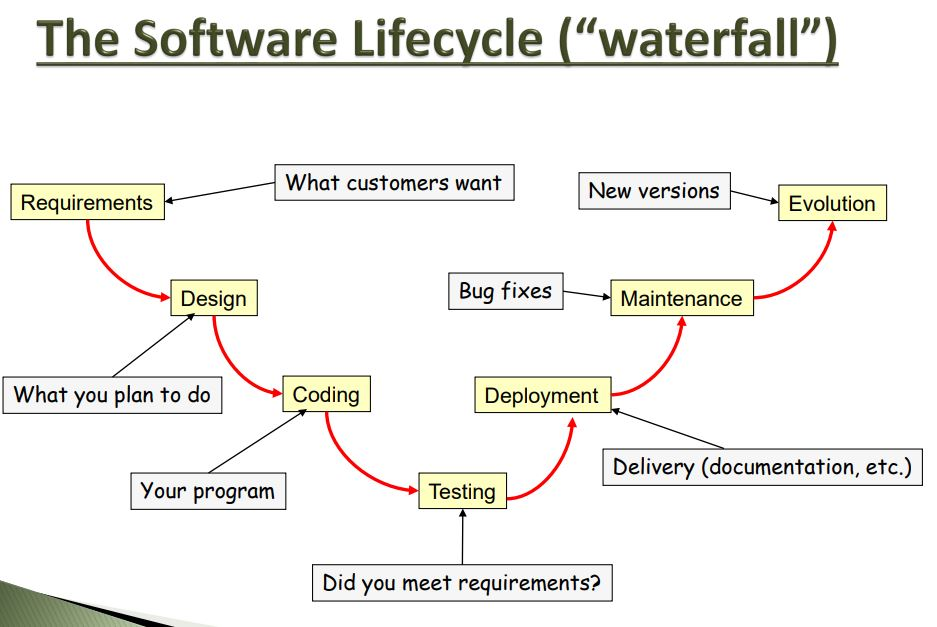
\includegraphics[scale=0.6]{media/lifecycle}
    \caption{Software Development Lifecycle}
    \label{fig:my_label}
\end{figure}

As shown above, software development typically starts by recognizing the requirements the software must satisfy. This consideration typically involves thinking about what customers want. Next, we go into the design phase in which we think about what we plan to do. Finally, we go into the coding phase, followed by testing, deployment, maintenance, and finally evolution. 

When developing software, it's also usually helpful to take a \vocab{top-down approach}. A top-down design is a method of ordering knowledge in which we start from a big idea (i.e. what we want to implement), and we break it down into what we need to achieve what's at the top (and we subsequently break those things down, and so on).


\vocab{Pseudocode} is also useful in creating software. Pseudocode is an English-like description of the set of steps required to solve a problem. Here's an example of some pseudocode for finding the minimum value from numerous inputted numbers.


\begin{center}
\line(1,0){400}
\end{center}

\begin{allintypewriter}

FIND\_MINIMUM \string{

\hspace{0.5cm} read the number of values to process; call this value N.

\hspace{0.5cm} repeat the following steps until N input values have been processed \string{

\hspace{1cm} read the next value into x

\hspace{1cm} if x is the first value read, set the current minimum to x.

\hspace{1cm} otherwise, if x is less than the current minimum, then set the current minimum to x.

\hspace{0.5cm} \string}

\string}

\begin{center}
\line(1,0){400}
\end{center}
\end{allintypewriter}

By using pseudocode, we can avoid having to deal with the subtleties of our programming language's syntax and semantics, and we can instead focus on determining the high-level steps necessary to solve a problem. %
\section{Wednesday, September 25, 2020}
Exam $1$ is today.%
\section{Friday, September 27, 2020}
Class is cancelled today due to a Football game.
\section{Monday, September 30, 2020}


\subsection{Introduction to Classes}

In Java, a \vocab{class} is a user-defined blueprint or protottype from which objects are created. Classes represent a set of properties or methods that are common to all objects of one particular type. They allow us to group together several variables and methods into one entity. \\

For instance, we can define a \verb!Superhero! class in one file called \verb!Superhero.java! as follows:

\begin{lstlisting}
public class Superhero {
    String name;
    int strength;
}
\end{lstlisting}

In this class, we've added a \verb!strength! and \verb!name! variable to represent the corresponding superhero's strength and name. Essentially, we've grouped together both of these variables into one entity (known as a \verb!Superhero!). Now, in another file, we can create instances of the \verb!Superhero! class: 

\begin{lstlisting}
public class Driver {
    public static void main(String args[]) {
        Superhero s1 = new Superhero();
        s1.name = "Batman";
        s1.strength = 100;
    }
}
\end{lstlisting}

We create a \verb!Superhero! object by using the \verb!new! keyword. In the driver program above, we've created a \verb!Superhero! object called \verb!s1!. When we create such an object, the object gets its own \verb!name! and \verb!strength! variables. We can access these variables present in the \verb!Superhero! class by using the dot operator (that is, we put a period after the variable, and we write the name of the variable that we want to access). As shown above, we've set our superhero's name to \verb!Batman!, and we've set its strength to $100$. \\

Classes can also have their own methods. For example, we can modify our \verb!Superhero.java! file to what follows below:

\begin{lstlisting}
public class Superhero {
    String name;
    int strength;
    
    void print() {
        System.out.println("Name: " + name);
        System.out.println("Strength: " + strength);
    }
}
\end{lstlisting}

Similar to how we access variables, we can access methods using the dot operator:

\begin{lstlisting}
public class Driver {
    public static void main(String args[]) {
        Superhero s1 = new Superhero();
        s1.name = "Batman";
        s1.strength = 100;
        s1.print(); /* This will print s1's name and strength. */
    }
}
\end{lstlisting}


Let's add another method:


\begin{lstlisting}
public class Superhero {
    String name;
    int strength;
    
    void print() {
        System.out.println("Name: " + name);
        System.out.println("Strength: " + strength);
    }
    
    void increaseStrength(int delta) {
        if (delta < 0) {
            System.out.println("Invalid strength increment.");
        } else {
            strength += delta;
        }
    }
}
\end{lstlisting}


Now, once we've instantiated a \verb!Superman! object, we can invoke the \verb!increaseStrength()! method in order to increase the superhero's strength (we don't want our users to be able to decrease the superhero's strength). \\


However, we are faced with a problem: nothing is stopping a user from simply setting the \verb!strength! variable of a \verb!Superman! object to a negative value (or a decreased value). Here's an example of what this means:


\begin{lstlisting}
public class Driver {
    public static void main(String args[]) {
        Superhero s1 = new Superhero();
        s1.name = "Batman";
        s1.strength = 100;
        /* s1's strength is 100. */
        s1.increaseStrength(-10);
        /* s1's strength is still 100. */
        s1.strength = 90; 
        /* s1's strength is 90. */
        System.out.println(s1.strength); /* Prints 90. */
    }
}
\end{lstlisting}

In order to overcome this issue, we can prevent our users from directly accessing the variables inside of a class by using the \vocab{private} keyword. By adding the keyword \verb!private! in front of the variables inside of our \verb!Superhero! class, we won't be able to use the dot operator to access them. Likewise, if we were to make our methods private, then they wouldn't be accessible from the outside (we don't want this, though). It's also a good idea to explicitly write \verb!public! before any of the variables or methods that we intend the user to have access to. \\

If we're making our variables private, then how do we set the variables of a \verb!Superhero! object? We can do so by simply creating a method that does this for us. Consider the following modified \verb!Superhero.java! file:

\begin{lstlisting}
public class Superhero {
    /* These variables can't be accessed with the dot operator. */
    private String name;
    private int strength;
    
    /* This method lets us set the values of our variables. */
    public void init(String nameIn, int strengthIn) {
        name = nameIn;
        if (strengthIn < 0) {
            System.out.println("Invalid strength.");
            strength = 0;
        } else {
            strength = strengthIn;
        }
    }
    
    public void print() {
        System.out.println("Name: " + name);
        System.out.println("Strength: " + strength);
    }
    
    public void increaseStrength(int delta) {
        if (delta < 0) {
            System.out.println("Invalid strength increment.");
        } else {
            strength += delta;
        }
    }
}
\end{lstlisting}

\noindent Now, we can update our driver program to the following:



\begin{lstlisting}
public class Driver {
    public static void main(String args[]) {
        Superhero s1 = new Superhero();
        // s1.name = "Batman" -> this won't compile; name is private.
        s1.init("Batman", 100); 
        // s1.strength = -1; -> this won't work; strength is private.
        s1.increaseStrength(5);
        // s1's stsrength is now 105.
    }
}
\end{lstlisting}

\subsection{Constructors}

Previously, we showed how we can limit a user's access to a class's variables --- by making the variables private, and providing public methods to set the variables. 

Since this is such a common thing to do, Java allows us to define a special method, known as a \vocab{constructor}, that is designed specifically for the purpose of setting up an object's variables upon instantiation. A constructor is declared by creating a method whose name is the same as the class's name. Moreover, this method is called when we're instantiating the object using the \verb!new! keyword. \\

Here's a modification of the \verb!Superhero! code that we saw earlier:

\begin{lstlisting}
public class Superhero {
    /* These variables can't be accessed with the dot operator. */
    private String name;
    private int strength;
    
    /* This is a constructor. */
    public Superhero(String nameIn, int strengthIn) {
        name = nameIn;
        if (strengthIn < 0) {
            System.out.println("Invalid strength.");
            strength = 0;
        } else {
            strength = strengthIn;
        }  
    }
    
    public void print() {
        System.out.println("Name: " + name);
        System.out.println("Strength: " + strength);
    }
    
    public void increaseStrength(int delta) {
        if (delta < 0) {
            System.out.println("Invalid strength increment.");
        } else {
            strength += delta;
        }
    }
}
\end{lstlisting}

The only thing that we've changed now is that we've replaced the \verb!init! method with a constructor. Now instead of invoking the \verb!init! method to instantiate our Superhero's variables, we can simply pass in the values we want ``on-the-fly" when we're instantiating the object:

\begin{lstlisting}
public class Driver {
    public static void main(String args[]) {
        Superhero s1 = new Superhero("Batman", 100);
        s1.print();
    }
}
\end{lstlisting}

When we execute \verb!Superhero s1 = new Superhero("Batman", 100);!, the \verb!name! and \verb!strenth! of \verb!s1! are set to Batman and $100$. There's also a special type of constructor, known as a \vocab{default constructor}, which is simply a constructor that takes in no arguments. One possible implementation of a default constructor for our \verb!Superman! class might look something like this:

\begin{lstlisting}
public class Superhero {
    /* Other code omitted. */
    
    /* Default constructor; takes in no arguments. */
    public Superhero() {
        strength = 0;
        name = "NONAME";
    }
}
\end{lstlisting}

Now, if we instantiate an object by calling \verb!Superman s1 = new Superman()!, it automatically gets assigned a strength of $0$, and a name of \verb!NONAME!. \\


There's another special method, known as the \verb!toString()! method, which simply tells the Java compiler what to print when we try to print the object. Currently, if we were to add the line \verb!System.out.println(s1);! into our program, our program would not compile. Why? Because \verb!System.out.println()! requires that we insert a string as the parameter. However, if we implement a \verb!toString()! method for the \verb!Superhero! object, then this line will compile, and it'll print whatever our \verb!toString()! method returns. \\

Here's what our modified code would look like:

\begin{lstlisting}
public class Superhero {
    /* These variables can't be accessed with the dot operator. */
    private String name;
    private int strength;
    
    /* This is a constructor. */
    public Superhero(String nameIn, int strengthIn) {
        name = nameIn;
        if (strengthIn < 0) {
            System.out.println("Invalid strength.");
            strength = 0;
        } else {
            strength = strengthIn;
        }  
    }
    
    public void increaseStrength(int delta) {
        if (delta < 0) {
            System.out.println("Invalid strength increment.");
        } else {
            strength += delta;
        }
    }
    
    public String toString() {
        String answer;
        answer = "Name: " + name;
        answer += ", Strength: " + strength;
        return answer;
    }
}
\end{lstlisting}

Now, we've gotten rid of our \verb!print()! method, and we've replaced it with a \verb!toString()! method. Instead of calling \verb!s1.print()!, we can instead call \verb!System.out.println(s1)!. % Fall 2018 video had no audio, so I used Fall 2017 video.

% October
\section{Wednesday, October 2, 2019}

Last time, we started talking about classes. Recall that classes can be \vocab{instantiated} using the \verb!new! keyword (for example, we can instantiate a \verb!Superhero! by writing \verb!Superhero s = new Superhero();!). An \vocab{object} is simply an instance of a class.

\subsection{.equals() method}

When we're implementing a class, sometimes it's useful to be able to be able to compare two instances of the class. In order to do so, there's a special function --- called \verb!.equals()! (``dot equals") --- that we can implement. Recall, for instance, that we use this method when we want to compare two strings (i.e. \verb!"Hello".equals("Hello")! evaluates to \verb!true!), which means that the \verb!String! class in Java implements the \verb!.equals()! method. \\

How does the \verb!.equals()! method work? Here's an example:

\begin{lstlisting}
public class Buffalo {
    public String name;
    public int age;
    
    public Buffalo(String name, int age) {
        this.name = name;
        this.age = age;
    }
    
    public Buffalo(int age) {
        this.age = age;
    }
    
    public boolean equals(Object obj) {
        if (obj == this) {
            return true;
        }
        if (obj == null || getClass() != obj.getClass()) {
            return false;
        }
        Buffalo buffalo = (Buffalo) other;
        return (this.name == other.age && this.age == other.age);
    }
    
}
\end{lstlisting}

Note that we've used a new keyword: \vocab{this}. The \textit{this} keyword can be used in Java as a reference to the current object. This is useful particularly when we have two variables of the same name, which allows us to get rid of ambiguity. \\

In the \verb!Buffalo! class above, we have implemented a method called \verb!equals! that returns a \verb!boolean!. Every time we create our own \verb!.equals()! method, we need to make sure that the function has the same function prototype (the return value and parameter list) as in this example. Moreover, the method needs to return \verb!true! if we deem the other object being passed in as a parameter to be equal to the current object, and it should return false otherwise. \\

How does our \verb!.equals()! method work?

\begin{itemize}
    \item First, we take in an object \verb!obj! as a parameter. We want to determine whether this object is equal to the current object that our class is representing.
    \item Firstly, we check if the parameter that we passed in \textit{is} the class that we're representing. This is done by, once again, using the \verb!this! keyword to obtain a reference to the current object. If the parameter passed in is the same as the class we're representing, then we know that the two objects must be the same.
    \item Next, we check whether the parameter is \verb!null!. If so, we return \verb!false! since we know that our current object isn't null, meaning that it cannot be equal to the parameter object. Moreover, we call \verb!getClass()! on our current object and the parameter object. This is a special function that Java provides for objects, and it tells us whether or not two objects have the same type. If they do not have the same type, then we can return false.
    \item At this point, we know that the two objects have the same type. Thus, we can treat the parameter object \verb!obj! as a \verb!Buffalo! object. This is done by casting the parameter as a \verb!Buffalo!. Finally, we can check the criteria that we want in order to check if the two \verb!Buffalo! objects are equal. In particular, we verify that the parameter object's name and age are equal to the current object's name and age. If they are, then we return \verb!true!; otherwise, we return \verb!false!.
\end{itemize}


Can we use the $\verb!.equals()!$ method without implementing it? Yes -- but it may not do what we want it to do. Every class, by default, has a \verb!.equals()! method. How does it work? It simply compares the two memory addresses of the variables we are using. In our \verb!Buffalo! example above, even if we set the \verb!name! and \verb!age! of two \verb!Buffalo! objects to the same values, we would end up finding that the default \verb!.equals()! method asserts that these two objects are different. In summary, it's not a good idea to rely on the default \verb!.equals()! method that Java provides for you.


\subsection{The ``this" Keyword}

Previously, we saw that we can use the \textit{this} keyword to obtain a reference to the current object. Here, we'll see a few more applications of the \verb!this! keyword. \\

Here is an implementation of a \verb!Person! class:

\begin{lstlisting}
public class Person {
    private String name;
    private int age;
    
    public Person(String name, int age) {
        this.name = name;
        this.age = age;
    }
    
    public Person(String name) {
        this(name, 18);
    }
    
    public person() {
        this("NONAME", 18);
    }
    
    public Person increaseAge(int delta) {
        age += delta;
        return this; /* Return reference. */
    }
}
\end{lstlisting}

\begin{itemize}
    \item In our first constructor, we use the \verb!this! keyword to reference the instance variables inside of our class. As mentioned previously, it can be useful to use this \verb!this! keyword here since our parameter variables have the same names as our instance variables. Using \verb!this! avoids ambiguity. 
    \item In our next two constructors, we use the \verb!this! keyword, almost like a function. What are these two lines doing? This is a special way to call one of the current object's constructors. In this case, since we've provided two parameters of type \verb!String! and \verb!int!, Java will recognize that we're trying to use the first constructor that we created. Thus, we set \verb!name! and \verb!age! according to the values that we provide in our \verb!this()! call. This is helpful since it allows us to reuse the code that we use in one constructor in another.
    \item Finally, in our \verb!increasingAge()! function, we return a reference to the current object by writing \verb!return this;!. This is allowed since our function prototype indicates that we're returning a \verb!Person!, and that's exactly what we're doing. 
\end{itemize}


Here's another example:

\begin{lstlisting}
public class HdTv {
    private String make;
    private int cost;
    
    public HdTv(String make, int cost) {
        this.make = make;
        this.cost = cost;
    }
    
    public HdTv(HdTv tv) {
        make = new String(tv.make);
        cost = tv.cost;
    }
    
    public String toString {
        return "Make: " + make + ", Cost: " + cost;
    }
    
    public static void main(String args[]) {
        HdTv tv = new HdTv("Poly", 100);
        System.out.println("Original--> " + tv);
        HdTv copy = new HdTv(tv);
    }
}
\end{lstlisting}

In this example, we introduce another application of the \verb!this! keyword: our \verb!HdTv! class implementation provides us with a constructor whose only parameter is another \verb!HdTv! object. The usefulness of this constructor is illustrated in our main method, where we initialize an \verb!HdTv! called \verb!copy! using another \verb!HdTv! called \verb!tv!. Such a constructor that uses an existing object to create a new object is known as a \vocab{copy constructor}.
\section{Friday, October 4, 2019}

\subsection{Breaking and Continuing}

In Java, we can use the \vocab{break} keyword to terminate the loop in which the \verb!break! statement is used (i.e. a for-loop, while-loop, or do-while loop). Here's an example:

\begin{lstlisting}
public class Example {
    public static void main(String args[]) {   
        int x = 0;
        while (true) {
            if (x == 40) {
                break; // Jump out of the loop.
            }
            x = x + 1;
            System.out.println(x);
        }
    }
}
\end{lstlisting}

How does this program work? At a first glance, it might seem like this program has an infinite loop --- we have a loop whose loop condition is just \verb!true!. However, as we've just mentioned, this while-loop includes a \verb!break! statement that gets executed when \verb!x! is equal to $40$. This \verb!break! statement will get us out of the loop after we print out the integers between $0$ and $39$, inclusive. \\

Can a \verb!break! statement be placed anywhere? No --- \verb!break! must be used either inside of a loop, or inside of a switch statement (which we will discuss later). If we place a \verb!break! statement somewhere that it is not supposed to be used, then we receive a compilation error. \\

What happens if we \verb!break! inside of a nested loop? We only exit the inner-most loop we're in (i.e. if we're inside of two for-loops, then we'll go outside of the innermost loop but inside of the outermost loop). \\

Next, we'll discuss the \vocab{continue} keyword in Java. The \verb!continue! keyword can be used inside of a loop to immediately jump to the next iteration of the loop. Here's an example:


\begin{lstlisting}
public class Example {
    public static void main(String args[]) {   
        int x = 0;
        while (true) {
            x = x + 1;
            if (x == 100) {
                break; // Jump out of the loop.
            }
            if (x % 2 == 0) {
                continue;
            }
            System.out.println(x);
        }
    }
}
\end{lstlisting}

What's happening here? Once again, we have a \verb!while (true) { ... }! loop. However, we can see that we're exiting the loop as soon as our variable \verb!x! becomes $100$. Also, we have now introduced a second conditional in which we check whether \verb!x! is an even number. If so, then we \verb!continue! onto the next iteration of the \verb!while! loop. Consequently, this program ends up printing all odd numbers between $1$ and $100$. \\


In general, one should be careful when using \verb!break! and \verb!continue! statements since they modify the control flow of the program. %
\section{Monday, October 7, 2019}

\subsection{Exceptions}

\subsection{Introduction}


When executing a program, oftentimes, something unexpected can happen. For instance, we might run out of memory, try to divide a number by $0$, or try to open a file that doesn't exist. \\

How do we recover from these unexpected occurrences? In Java, we can perform  \vocab{exception handling}. An \vocab{exception} is an event that occurs during the execution of a program that disrupts the normal flow of instructions (the examples listed previously are all examples of exceptions). Exception handling lets us recover in the case that an exception occurs. \\


To illustrate an example, consider the following program:

\begin{lstlisting}
public class MilesPerGallon {
    public static void main(String args[]) {
        Scanner scanner = new Scanner(System.in);
        System.out.println("Enter numbre of gallons: ");
        int miles = scanner.nextInt();
        
        System.out.println("Enter number of gallons: ");
        int gallons = scanner.nextInt();
        
        int milesPerGallon = miles / gallons;
        
        System.out.println("Miles per gallon is " + milesPerGallon);
        
        scanner.close();
\end{lstlisting}

In this program, we let the user provide integer values for the number of miles and the number of gallons that they use, and we subsequently divide the two quantities to find the miles per gallon used. But, what happens if the user enters the value $0$ for \verb!gallons!? We get an exception when we try to compute \verb!milesPerGallon! (since we're trying to divide by $0$). \\

One way to solve this issue is to simply use an \verb!if-else! statement to check whether the user's input is $0$. But, what happens if there are several ``bad" values that we want to be careful of (in this case, the only ``bad" value to be careful of is $0$, but if there were too many, then it might not be feasible to enumerate them all)? In this scenario, we would need to use exception handling. \\

One way in which we can handle exceptions is by using a \verb!try-catch! block. In Java, a \verb!try! statement lets us define a block of code to be tested for errors while it is being executed. Furthermore, the \verb!catch! block can be used to define a block of code to be executed, if an error occurs in the \verb!try! block. Here's the same code from above, but now written with a \verb!try-catch! block: 

\begin{lstlisting}
public class MilesPerGallon {
    public static void main(String args[]) {
        Scanner scanner = new Scanner(System.in);
        System.out.println("Enter numbre of gallons: ");
        int miles = scanner.nextInt();
        
        System.out.println("Enter number of gallons: ");
        int gallons = scanner.nextInt();
        try {
            int milesPerGallon = miles / gallons;
        
            System.out.println("Miles per gallon is " + milesPerGallon);
        } catch (ArithmeticException e) {
            System.out.println("Invalid value provided!");
            System.out.println("Default message: " + e.getMessage());  
        }
        System.out.println("Thank you for using our system.");
        scanner.close();
\end{lstlisting}

In the code above, we can note the following changes:

\begin{itemize}
    \item We've placed the \verb!int milesPerGallon = miles / gallons;! statement in the \verb!try! block that we've created. Why? Because this is the portion of code that might result in an exception. More precisely, the exception that we want to avoid is known as an \verb!ArithmeticException! (this is the name of the exception that results from trying to divide by zero).
    \item Next, we've added a \verb!catch (..) { ... }! block. Inside of the parentheses directly after the \verb!catch! statement, we need to specify what type of exception we want to watch out for. In this case, we've specified that we want to watch out for \verb!ArithmeticException!s since this type of exception takes place when we try to divide by zero. Is it possible to watch out for \textit{all} exceptions? Yes --- instead of specifying the specific type of exception, like \verb!ArithmeticException!, we would just write \verb!Exception!. 
    \item Inside of the \verb!catch! block, we specfy the instructions that we want to execute if an exception takes place. In our program, we simply notify the user that they've proivded an invalid value. Moreover, we print the message associated with the \verb!ArithmeticException! exception by calling the \verb!.getMessage()! method on it. 
    \item Finally, we print ``Thank you for using our system," outside of the \verb!try-catch! block. This message gets printed regardless of what the user inputs. Finally, we close our scanner, and we're done. 
\end{itemize}

In Java, exceptions are represented by \textit{objects}. Java has a built-in class called \verb!Exception!, and we can treat an \verb!Exception! as an object. This is seen clearly in the example above, where we call the \verb!.getMessage()! method associated with the \verb!ArithmeticException! object \verb!v!.  \\

If a user ever provides the value $0$ for \verb!gallons!, then we jump out of the \verb!try! block as soon as the exception takes place. This means that the statement \verb!System.out.println("Miles per gallon is " + milesPerGallon);! is \textit{never executed}. 
Here are some of the most common types of exceptions that we should be wary of:

\begin{itemize}
    \item \verb!ArithmeticException! is an exception that occurs when we try to divide by zero (like in the example above).
    \item \verb!NullPointerException! occurs when we attempt to acces an object with a null reference.
    \item \verb!IOException! occurs when we attempt to perform illegal input/output operations.\verb!IndexOutOfBoundsException! occurs when we attempt to access part of an array (which we will introduce later) or \verb!String! outside of the range in which it's defined.
\end{itemize}


\subsection{Exception Propagation}

When an exception takes place, Java always looks in the current method for a catch clause that matches the exception. If one is found, the exception is handled using that \verb!try-catch! block. Otherwise, \vocab{exception propogation} takes place. \\

What is exception propogation? When an exception occurs, Java pops back up the call stack (e.g. goes up through the various methods it is nested in) to see whether the exception is being handled in a catch block of one of the methods. This process is known as exception propogation. The first method that handles the exception defines how we handle the exception. If we get all the way back up to the \verb!main! method and no method catches the exception, then Java will abort your program. \\

Here's an example:

\begin{lstlisting}
public class Propagation {
	public static void B() {
		Scanner scanner = new Scanner(System.in);

		System.out.println("Enter number of miles: ");
		int miles = scanner.nextInt();

		System.out.println("Enter number of gallons: ");
		int gallons = scanner.nextInt();

		int milesPerGallon = miles / gallons;
		System.out.println("Miles per gallon is: " + milesPerGallon);

		scanner.close();
	}

	public static void A() {
		System.out.println("Before calling method B");
		B();
		System.out.println("After calling method B");
	}

	public static void main(String[] args) {
		try {
			System.out.println("Before calling method A");
			A();
			System.out.println("After calling method A");
		} catch (ArithmeticException e) {
			System.out.println("Invalid value provided");
			System.out.println("Default Message: " + e.getMessage());
		}
		System.out.println("Thank you for using our system");
	}
}
\end{lstlisting}

In the following code, we note that our ``dangerous code," which might cause an exception, has now been moved to the function \verb!B()!. However, we've introduced another function called \verb!A()!, which simply prints a statement, calls the function \verb!B!, and prints another statement. \\

In our \verb!main! method, we have a \verb!try-catch! block in which we print a statement prior to calling \verb!A!, call \verb!A!, and subsequently print another statement. \\

What happens if the user of the program enters $0$ for the number of miles? Even though our function \verb!B! does not have a \verb!try-catch! block, error propagation will occur since the exception is being thrown inside of a function. More precisely, once we try to divide by $0$, we'll check ``up one level" for a \verb!try-catch! block. Since the function \verb!A! doesn't have a  \verb!try-catch! block either, we'll go up again into the \verb!main! method. In the \verb!main! method, we'll find a \verb!try-catch! block, and we'll perform the error handling in the \verb!catch! block. \\

What happens if we add another \verb!try-catch! block in \verb!A!? Then the \verb!try-catch! block in \verb!A! will be used instead of the \verb!try-catch! block in the main (we always use the \verb!try-catch! block that's closest to the error on the stack). \\

What happens if we \textit{remove} the \verb!try-catch! block in the \verb!main! method? Our program will abort with an exception when we try to divide by $0$. 


\subsection{Throwing Exceptions}

So far, we've seen how to handle exceptions. However, it turns out that we can throw our own exceptions as well. Why would we want to do this? Mainly because it helps us debug; by throwing an exception when something goes wrong, we know exactly what went wrong, and we can figure out how to fix the issue. \\

The general syntax to throw an exception is shown below:

\[
\verb!throw new [ExceptionName](message);!
\]


One instance in which it's useful to throw an exception is when we haven't implemented a method yet:

\begin{lstlisting}
	public static double computeCost(int option) {
		throw new UnsupportedOperationException("Not implemented yet");
	}
\end{lstlisting}

In the code segment above, we don't have an implementation of the \verb!computeCost! method yet, so we just throw an exception instead. This is helpful since it allows our code to still compile (we don't need to comment out this method until we implement it). Furthermore, if a user tries to call this method, then they will receive a message telling them that the method is not implemented yet. \\


Here's another example in which the usefulness of throwing exceptions is clear:

\begin{lstlisting}
    	public static int processCourse(String courseName) {
		if (courseName == null) {
			throw new IllegalArgumentException("Invalid argument");
		} else {
			if (courseName.equals("cmsc131")) {
				return 4;
			} else {
				return 1;
			}
		}
	}
\end{lstlisting}

In this method, we throw an \verb!IllegalArgumentException! if the user provides a \verb!null! reference to a \verb!String! object.  Once again, this is very helpful since it tells us right away what the issue is, and we don't have to spend long periods of time searching for the error. % 
\section{Wednesday, October 9, 2019}


\subsection{``Finally" Blocks}

Last time, we introduced \verb!try-catch! blocks, which are used to handle exceptions. Today, we'll introduce the \vocab{finally} keyword. A \verb!finally! block is typically used along with a \verb!try-catch! block. The purpose of a finally block is to hold all of the crucial statements that must be executed, whether the exception occurs or not. The statements present in the \verb!finally! block will \textbf{always} execute, regardless of whether an exception occurs or not. \\

\noindent Here's an example:

\begin{lstlisting}
	public static int getGasAverage() {
		Scanner scanner = new Scanner(System.in);

		System.out.println("Enter number of miles: ");
		int miles = scanner.nextInt();

		System.out.println("Enter number of gallons: ");
		int gallons = scanner.nextInt();

		try {
			int milesPerGallon = miles / gallons;
			System.out.println("Miles per gallon is: " + milesPerGallon);
			
			return milesPerGallon;
		} finally {
			scanner.close();
			System.out.println("Before leaving method getGasAverage() (finally message)");
		}
	}

	public static void main(String[] args) {
		try {
			System.out.println("Before calling method getGasAverage() (main)");
			System.out.println("Average: " + getGasAverage());
			System.out.println("After calling method getGasAverage() (main)");
		} catch (ArithmeticException e) {
			System.out.println("Invalid value provided (in main)");
			System.out.println("Default Message: " + e.getMessage());
		}
		System.out.println("Thank you for using our system");
	}
\end{lstlisting}

What's happening here?

\begin{itemize}
    \item In main method, we have a \verb!try-catch! block in which we call the function \verb!getGasAverage()!. In our \verb!getGasAverage! function, we read in the \verb!miles! and \verb!gallons! variables using a scanner.
    \item In the \verb!getGasAverage! function, we have another \verb!try-catch! block in which we divide the \verb!miles! by \verb!gallons!. What happens if the user provides the value $0$ for \verb!gallons!? An exception is thrown, and Java starts searching for a \verb!catch! block. Since there's no \verb!catch! block in the \verb!getGasAverage! function, we use the \verb!catch! block in the main.
    \item After executing the \verb!catch! block in the \verb!main! method, we execute the code in \verb!finally!. Recall that the statements in \verb!finally! blocks are \textit{always} executed. 
    \item Inside of the \verb!finally! block, we close the scanner. Note that this is something that we always want to do when we're done with the scanner, whether an exception took place or not. 
\end{itemize}

In the code segment above, we have a \verb!try { ... } finally { ... }! block inside of our \verb!getGasAverage()! method; however, we are also permitted to have \verb!try { ... } catch (..) { .. } finally { ... }! blocks. \\

In summary, the \verb!finally! keyword allows us to group together some statements that should \textit{always} be executed, whether an exception is thrown or not. Often, these instructions might include closing a scanner, closing a file, or printing some message.

\subsection{String Methods}

In Java, the \verb!String! class has several built-in methods that are readily usable on strings. Today, we'll discuss some of the most commonly used ones. 


\begin{itemize}
    \item The \verb!.charAt()! method takes in an single integer as a parameter, and it returns the character at the given index (starting from $0$). For example, \verb!"Hello".charAt(0)! would return \verb!H!, and \verb!"Hello".charAt(1)! would return $e$
    \item The \verb!.length()! method returns the number of characters in the \verb!String! (where we start counting from $1$). For instance, \verb!"Hello".length()! returns $5$.
    \item \verb!.toLowerCase()! and \verb!.toUpperCase()! return another String variable with all of the letters in the \verb!String! in lowercase or in uppercase. For example, \verb!"Hello".toLowerCase()! returns \verb!hello!, whereas \verb!"Hello".toUpperCase()! returns \verb!HELLO!. Since strings are immutable, these methods return entirely new objects.
\end{itemize}

There are several other String methods available to us as well. A full list is available in the Java API at \url{https://docs.oracle.com/javase/7/docs/api/java/lang/String.html}. \\

Here's a sample program that illustrates how some of these methods work:

\begin{lstlisting}
package apisEx;

import javax.swing.*;

public class StringExamples {
	public static void main(String[] args) {

		String name = JOptionPane.showInputDialog("Enter a word");
		String answer;

		if (name.charAt(0) == name.charAt(name.length() - 1)) {
			answer = "word starts and end with the same letter";
		} else {
			answer = "word does not start and end with the same letter";
		}
		JOptionPane.showMessageDialog(null, answer);

		String str1 = JOptionPane.showInputDialog("Enter string");
		String str2 = JOptionPane.showInputDialog("Enter string");
		System.out.println("Using compareTo: " + str1.compareTo(str2));
		System.out.println("Using compareToIgnoreCase: " + str1.compareToIgnoreCase(str2));

		String login = JOptionPane.showInputDialog("Enter login id");
		answer = "Access Granted";
		if (!login.equalsIgnoreCase("Hulk")) {
			answer = "Access Denied";
		}
		JOptionPane.showMessageDialog(null, answer);

		String mascot = " Terps ";
		System.out.println("Character r for Terps is at : " + mascot.indexOf('r'));
		System.out.println("Before trimming:--" + mascot + "--");
		String mascotTrimmed = mascot.trim();
		System.out.println("After trimming:--" + mascotTrimmed + "--");
		System.out.println("Uppercase: " + mascot.toUpperCase());
		System.out.println("Lowercase: " + mascot.toLowerCase());
		System.out.println("Mascot after trimming and case changes:--" + mascot + "--");

		int x = 100;
		String strIntValue = String.valueOf(x);
		System.out.println(strIntValue);
	}
}
\end{lstlisting}

In this example, we also introduce the \verb!JOptionPane! class, which is simply a way to produce graphical user interfaces. This can be used to make our programs more interactive; however, it would also be fine to just use a \verb!Scanner!. \\


In this example, we read in the variable \verb!name! from the user's input. On Line $11$, we call \verb!.charAt(0)! to retrieve the first character of the user's inputted string, and we call \verb!.charAt(name.length() - 1)! to retrieve the last character of the user's inputted string. If these two characters are the same, then we display the message ``word starts and ends with the same character." \\

Next, we read in two more strings, and we display what the \verb!.compareTo()! and \verb!.compareToIgnoreCase()! methods return. Recall that the \verb!.compareTo()! method returns the integer $0$ if the two strings are equal, a positive value if the first string is lexicographically greater than the second string, and a negative number otherwise. On the other hand, the \verb!.compareToIgnoreCase()! function does the exact same, while ignoring the case of each character (\verb!A! is considered the same as \verb!a!, etc). \\

\subsection{Math Methods}

Now, we'll introduce some useful math methods that we can use. Here are some of the most common methods that are made available to us:

\begin{itemize}
    \item The \verb!Math.abs()! method takes in a number, and it returns the absolute value of that value. For example, \verb!Math.abs(5) = 5!, and \verb!Math.abs(-5) = 5!. 
    \item The \verb!Math.ceil()! method takes in a double, and it returns the ceiling (smallest integer larger than the number) of the number. For example, \verb!Math.ceil(3.5) = 4!, and \verb!Math.ceil(5) = 5!
    \item The \verb!Math.floor()! method takes in a dobule, and it returns the floor (largest integer less than the number) of the number. For example, \verb!Math.floor(3.5) = 3!, and \verb!Math.floor(3) = 3!. 
    \item The \verb!Math.pow()! method takes in two values, and it returns the first argument raised to the power of the second argument. For example, \verb!Math.pow(2, 3)! evaluates to $2^{3} = 8$. 
\end{itemize}


\noindent Here's a Java program illustrating some of these methods:

\begin{lstlisting}
public class MathExamples {
	public static void main(String[] args) {

		// Math m = new Math(); // not possible
		System.out.println("Math.PI: " + Math.PI);
		System.out.println("Maximum between 20 and 10: " + Math.max(20, 10));
		System.out.println("Minimum between 20 and 10: " + Math.min(20, 10));

		double value = Double.parseDouble(JOptionPane.showInputDialog("Enter number"));
		System.out.println("Square root of " + value + ": " + Math.sqrt(value));
		System.out.println("Floor of " + value + ": " + Math.floor(value));
		System.out.println("Ceiling of " + value + ": " + Math.ceil(value));
		System.out.println("Power (2) of " + value + ": " + Math.pow(value, 2));
		System.out.println("Rounding " + value + ": " + Math.round(value));

		System.out.println("Set 1");
		for (int i = 0; i < 100; i++) {
			System.out.println(Math.random());
		}

		System.out.println("Set 2");
		for (int i = 0; i < 100; i++) {
			System.out.println(200 * Math.random());
		}

		System.out.println("Set 3");
		for (int i = 0; i < 100; i++) {
			System.out.println(Math.floor(200 * Math.random()));
		}

		System.out.println("Set 4");
		for (int i = 0; i < 100; i++) {
			System.out.println(Math.floor(201 * Math.random()));
		}

		System.out.println("Set 5");
		for (int i = 0; i < 100; i++) {
			System.out.println(Math.floor(200 * Math.random()) + 1);
		}
	}
}
\end{lstlisting}

Here are some useful observations that we can make:

\begin{itemize}
    \item First, we read in a \verb!double! on Line $9$. Line $10$ prints out the square root of the number, Line $11$ prints out the floor of the number, Line $12$ prints out the ceiling of the number, Line $13$ prints out the square of the number, and Line $14$ rounds the number.
    \item On Line $18$, we print out \verb!Math.random()! $100$ times. What does \verb!Math.random()! do? It returns a pseudorandom number on the interval $[0, 1]$. 
    \item In the subsequent for-loops, we shift our interval \verb![0, 1]! to various other intervals so that we can generate random numbers in any interval we want. For example, if we add a constant value $c$ to \verb!Math.random()!, then we end up generating values in the interval \verb![c, 1 + c]!. Moreover, we can scale the interval by multiplying it by different values.
\end{itemize}%
\section{Friday, October 11, 2019}

\subsection{Immutable Classes}

In Java, an \vocab{immutable class} is a class whose content we cannot change. Recall that the \verb!String! class in Java is immutable. Why is immutability good? Because they make our code more safer and cleaner, which is particularly important when we are multithreading. \\

The \vocab{final} keyword in Java can be used before a variable to prevent it from being changed. The only place in which we can assign a value to a \verb!final! variable is inside of a constructor. After the constructor is executed, a \verb!final! variable cannot be changed. \\



Here's an example of an immutable class:

\begin{lstlisting}
public final class Telephone {
	private final String number;

	public Telephone(String number) {
		this.number = number;
	}

	public String getNumber() {
		return number;
	}

	public String toString() {
		return "Telephone [number=" + number + "]";
	}

	public static void main(String[] args) {
		Telephone telephone = new Telephone("1-899-COMPILE_JAVA");

		System.out.println(telephone);
	}
}
\end{lstlisting}

In the code segment above, we've also specified our class as \verb!final!. Declaring a class as final prevents it from being extended, which is something that we will discuss later. In the code above, we've declared both our class and our \verb!number! variable as \verb!final!. This is an example of an immutable class since, once an object is created, it cannot be modified.  \\

\subsection{Ternary Operator}

In Java, the \vocab{ternary operator} is an operator that takes in three arguments. The first argument is a Boolean condition, the second argument is the result that the operator should return if the condition evaluates to true, and the third condition is the result that the operator should return if the condition evaluates to false. \\

The ternary operator might look confusing, but with a few examples, it is not too hard to understand. The general form of the ternary operator is shown below:

\[
\verb!condition ? exprValueIfConditionIsTrue : exprValueIfConditionIsFalse!
\]

Here's an example:

\begin{lstlisting}
public class Example {
    public static void main(String args[]) {
        
        Scanner scan = new Scanner(System.in);
        int x = scan.nextInt();
        int y = scan.nextInt();
        int ans = (x > y) ? x : y;
        System.out.println("Maximum is " + ans);
        scan.close();
    }

}
\end{lstlisting}

What's this program doing? First, we just declare a scanner, and we read in two integer variables \verb!x! and \verb!y!. Next, we initialize the variable \verb!ans! using the ternary operator. Here, our condition is the Boolean expression \verb!(x > y)!. If this Boolean expression evaluates to \verb!true!, then we set \verb!ans! equal to \verb!x!; otherwise, we set \verb!ans! equal to \verb!y! In other words, we are simply setting \verb!ans! to the maximum of the two variables that we are reading in. \\

We could easily change our initialization of \verb!ans! to 

\[
\verb!int ans = (x < y) ? x : y;!
\]

if we wanted \verb!ans! to store the minimum value instead. \\

It might be helpful to think of the ternary operator as a shortened way of writing an if-else statement. If the condition provided is true, then we evaluate the ternary expression to the first expression provided; otherwise, we evaluate it to the second expression provided. 

\subsection{The Switch Statement}

A \vocab{switch} statement in Java allows a variable to be tested for equality against a list of several values. Each value in the list is called a \vocab{case}, and the variable being ``switched on" is checked for each case. \\

Pretty much, a \verb!switch! statement is a more convenient --- and often more efficient --- way to perform a multi-way conditional based on a single control value. \\

The general syntax of a \verb!switch! statement is as follows:


\begin{lstlisting}
switch (variable) {
    case 1:
        System.out.println("Case 1!");
        break;
    
    case 2:
        System.out.println("Case 2!");
        break;
        
    // ... ... ....
    
    default:
        System.out.println("Invalid");
        break;
}
\end{lstlisting}

The \verb!switch! statement code presented above would be equivalent to the following code:

\begin{lstlisting}
if (variable == 1) {
    System.out.println("Case 1!");
} else if (variable == 2) {
    System.out.println("Case 2!");
    // ... .... ..
} else {
    System.out.println("Invalid!");
}
\end{lstlisting}

The case that is selected in a \verb!switch! statement is dependent on the value of the \verb!variable!. The \verb!break! statement within each case is used to exit the \verb!switch! statement afterwards.


Here's a fully working example:

\begin{lstlisting}
public class SwitchExample {
	public static void printDay(int day) {
		String answer;

		switch (day) {
		case 6:
			answer = "Saturday";
			break;
		case 1:
		case 2:
		case 3:
		case 4:
		case 5:
			answer = "Weekday";
			break;
		case 7:
			answer = "Sunday";
			break;
		default:
			answer = "Invalid day value";
			break;
		}
		System.out.println("Value " + day + " corresponds to " + answer);
	}

	public static int printYear(String type) {
		int year;

		switch (type) {
		case "Freshman":
			year = 1;
			break;
		case "Sophomore":
			year = 2;
			break;
		case "Junior":
			year = 3;
			break;
		case "Senior":
			year = 4;
			break;
		default:
			year = -1;
			break;
		}

		return year;
	}

	public static void main(String[] args) {
		Scanner scanner = new Scanner(System.in);

		System.out.println("Enter integer value for day of the week: ");
		int day = scanner.nextInt();
		printDay(day);

		System.out.println("Enter student's classification: ");
		System.out.println(printYear(scanner.next()));

		scanner.close();
	}
}
\end{lstlisting}

Here's what's happening:

\begin{itemize}
    \item In the main method, we first read in an integer from the user, and we store it in the variable \verb!day!. Next, we call our function \verb!printDay()! with \verb!day! as an input parameter.
    \item In our \verb!printDay()! method, we utilize a switch statement. The variable that is being switched on is \verb!day!. In each case, we compare the value of \verb!day! to the case number (first, we compare \verb!day! to $6$, then we compare it to $1$, and so on). 
    \item If \verb!day! is equal to $6$, then we set \verb!answer! equal to \verb!Saturday!, and we break out of the switch statement. If \verb!day! is equal to $1, 2, 3, 4, \text{ or } 5$, then we set \verb!answer! equal to \verb!Weekday!, and we break out of the \verb!switch! statement.
    \item If \verb!day! has any other value, then we set \verb!answer! to \verb!Invalid day value!, and we break out of the \verb!switch! statement.
    \item Finally, we print out the value of \verb!day!, and we print out the \verb!answer! string that we stored. 
\end{itemize}

The \verb!printYear! function works in a similar manner; however, it demonstrates that \verb!switch! statements don't only have to be used with integers --- they can be used with strings as well. %
\section{Monday, October 14, 2019}

Today, we'll start talking about arrays.

\subsection{Arrays}

Suppose we have a \verb!Student! class, and we want to keep track of three students. From what we've learned so far, we could just initialize three \verb!Student! variables. But what happens if we need to keep track of $100$ students? Or $10,000$ students? Clearly, our current method is not feasible. This is where arrays come into picture. \\

An \vocab{array} in Java is an object used to store a fixed-size sequential collection of elements of the same type. The benefits of an array is that we can treat an array as a single entity, but we can also access each of the individual elements that are stored inside of the array. \\

How do we declare an array? We can declare an array of a given type with the general format:

\[
\verb!type[] variablename;!
\]

For example, we can declare an array of \verb!int!s named \verb!arr! by simply writing \verb!int[] arr;!. Similarly, we can create an array of characters by writing \verb!char[] arr;!. \\

How do we initialize an array? We use the \verb!new! keyword, we respecify the type, and we finally specify the size of the array. The general syntax is provided below:

\[
\verb!type[] variablename = new type[size];!
\]

For example, if we want to declare an array of $10$ integers, then we can write,

\[
\verb!int[] arr = new int[5];!
\]

\noindent The code above would initialize an array of $5$ \verb!int!s, and we would now have $5$ \verb!int!s at our disposal. By default, the values of an \verb!int! array are all initialized to $0$. We view an array as a a contiguous block in memory, so we might visualize \verb!arr! as follows:

\[
\fbox{0} \sep \fbox{0} \sep \fbox{0} \sep \fbox{0} \sep \fbox{0}
\]

\noindent We can access each of the individual \verb!int! values in our array by writing the name of the array, followed by square brackets, with a number corresponding to the entry that we wish to access (starting from $0$). For example, we can change the first value in our array by writing \verb!arr[0] = 5;!, and we can change the last element in our array as \verb!arr[4] = 7;!. Afterwards, our array will look like the following:

\[
\fbox{5} \sep \fbox{0} \sep \fbox{0} \sep \fbox{0} \sep \fbox{7}
\]

\noindent The process of accessing an individual element in an array is called \vocab{indexing}. 

Here's some code illustrating some of the nice things that we can do with arrays:

\begin{lstlisting}
public class ReadValues {

	public static void main(String[] args) {
		Scanner scanner = new Scanner(System.in);

		System.out.println("How many values would you like to store: ");
		int size = scanner.nextInt();

		int[] nums = new int[size];

		for (int i = 0; i < nums.length; i++) {
			System.out.println("Enter value " + (i + 1) + ": ");
			nums[i] = scanner.nextInt();
		}

		System.out.println("Here are the values you entered:  ");
		for (int i = 0; i < nums.length; i++) {
			System.out.println(nums[i]);
		}

		scanner.close();
	}
}
\end{lstlisting}

A summary of what's going on in this code is presented below:

\begin{itemize}
    \item Firstly, we ask our user to enter the number of values they want to store. We read in this value, and we initialize an array with that size.  
    \item Next, we read in the corresponding number of values by using a for-loop. In each iteration of the for-loop, we ask the user to enter the next value, and we store it into the next entry in the array. Note that our array has a built-in \verb!.length! field that we can access. This is simply an integer variable that tells us the size of the array.
    \item Finally, we use another for-loop to iterate over our array. In the \verb!i!th iteration of the for-loop, we print \verb!nums[i]!, which is the \verb!ith! element in our array. 
\end{itemize}

It's important to note that arrays start at $0$. This means that, if we're storing $10$ elements, then it's only valid to access the array at the indices $0, 1, 2, \ldots, 9$. What happens if we try to access an element that's out of bounds? An exception is thrown, and our Java program will abort if we don't have a \verb!try-catch! block. 


To summarize, there are three different situations that we've learned so far in which we can use the square brackets \verb![..]!. 

\begin{enumerate}
    \item Firstly, we use square brackets when we're trying to declare an array (e.g. \verb!int[] arr;!).
    \item We also use square brackets when we're initializing an array (i.e. \verb!arr = new int[10];)!.
    \item Finally, we also use square brackets when indexing an array (i.e. \verb!arr[0]! accesses the first element, \verb!arr[1]! accesses the second element, and so on).
\end{enumerate}

\subsection{Copying Arrays}

Consider the following code segment:

\begin{lstlisting}
public class Example {
    public static void main(String args[]) {
        int[] a = new int[5];
        for (int i = 0; i < 5; i++) {
            a[i] = i;    
        }
        int[] b = a;
    }
}
\end{lstlisting}

First, we initialize a variable \verb!a!. Subsequently, we use a for-loop, and we set \verb!a[i]! equal to \verb!i! for $i = 0, 1, 2, 3, 4$.  Next, we create a new variable called \verb!b!, and we set it equal to \verb!a!. 

Would this copy the elements of \verb!a! into \verb!b! (does \verb!b! contain the elements $0, 1, 2, 3, 4$)? The answer is no --- this just makes \verb!a! and \verb!b! aliases for each other. This is similar to creating a \verb!String! variable, and setting a new \verb!String! variable equal to it. \\

So how do we copy the contents of \verb!a! into \verb!b!? We need to use a for-loop and iterate over the elements of \verb!a!, while assigning the \verb!i!th element of \verb!a! to \verb!b[i]!. This is shown below:

\begin{lstlisting}
public class Example {
    public static void main(String args[]) {
        int[] a = new int[5];
        
        for (int i = 0; i < 5; i++) {
            a[i] = i;
        }
        
        int[] b = new int[5];
        /* Copy contents of a into b. */
        for (int i = 0; i < a.length; i++) {
            b[i] = a[i];
        }
    }
}
\end{lstlisting}% Missing random numbers.
\section{Wednesday, October 16, 2019}

Today, we'll continue talking about arrays.

\subsection{Resizing Arrays}

When we initialize an array with a fixed size, this size cannot be changed. For example, the following code will not compile:

\begin{lstlisting}
public class Example {
    public static void main(String args[]) {
        int arr[] = new int[10]; /* Declare an array of size 10. */
        arr.length += 5; /* THIS DOESN'T WORK! */
    }
}
\end{lstlisting}

We cannot increment the \verb!length! variable associated with an array; it is declared as a constant variable with the \verb!final! keyword. So, how do we resize an array? We need to create a completely new array, and copy over the elements. 

\subsection{Arrays of References}

%
\section{Friday, October 18, 2019}

\subsection{Array Initialization Lists}
Suppose we want to create an array with the integers one through five. One way of doing so would be writing, \verb!int arr[] = new int[5]! and subsequently setting \verb!arr[0]!, \verb!arr[1]!, and so on to their respective values. Alternatively, one might use a loop to set each value. \\

Although it isn't possible to assign all of the elements at once, it is often helpful to use \vocab{initialization lists}, which allow us to create arrays ``on-the-fly." Arrays can be initialized at declaration time by explicitly writing the values enclosed in curly brackets. Thus, instead of the two solutions described above, we could instead just write 
\[
\verb!int arr[] = {1, 2, 3, 4, 5}!. 
\]

In fact, we can also use this syntax to only declare a few elements in the array. If there are fewer initializers than elements in the array, then the remaining elements are automatically initialized to zero. For example, writing \verb!int arr[10] = {1, 2, 3, 4, 5}! would set the first five elements to $1, 2, 3, 4,$ and $5$, but the last five elements would be set to zero (if we don't specify the size of the array in the square brackets, then the length of the array will just be equal to the number of elements we explicitly put in the initializer list).

We can only use an initialization list in the form described above when we're declaring a variable. It wouldn't be valid, for instance, to pass an initialization list to a method. However, we can also create arrays on-the-fly with the following syntax, which can be passed into parameters: 

\[
\verb!int arr[] = new int[]{1, 2, 3, 4, 5};!
\]

Although we've only shown initialization lists for \verb!int! variables here, they are valid for any type. \\


Here's an example:

\begin{lstlisting}
public class PassingArrays {
    public void printArray(int[] arr) {
        for (int i = 0; i < arr.length; i++) {
            System.out.println(arr[i] + " ");
        }
        System.out.println();
    }
    
    public static void main(String args[]) {
        printArray(new int[]{5, 78, 4});
    }
}
\end{lstlisting}

Note that this is convenient because it saves us the time of creating a new array and setting each value individually when we aren't planning to use the array ever again.

\subsection{Arrays in Classes}

We've already seen that classes have instance variables, which represent the entities associated with the class. Classes can also have references to arrays, which can be useful at times.

Before we demonstrate an example of a class that has a reference to an array, we'll first take a look at the following \verb!Student! class:

\begin{lstlisting}
package rosterExample;

public class Student {
	private String name;
	private int score;
	
	/**
	 * 
	 * @param name
	 * @param score value between 0 and 100
	 */
	public Student(String name, int score) {
		this.name = name;
		this.score = score;
	}

	/**
	 * 
	 * @return student's score
	 */
	public int getScore() {
		return score;
	}

	/**
	 * 
	 * @param score
	 */
	public void setScore(int score) {
		this.score = score;
	}

	public String toString() {
		return "name: " + name + ", score: " + score;
	}
}
\end{lstlisting}

The \verb!Student! class above simply represents a student in a class. Each student has a \verb!name! and a \verb!score!. 

Now, we'll take a look at the following \verb!Roster! class, which is used to represent a class's roster of students. This class illustrates how having the an array's reference can be useful: 

\begin{lstlisting}
package rosterExample;

/**
 * Represents a class rosters.
 * @author cmsc131
 *
 */

public class Roster {
	public static final String SCHOOL = "UMCP";
	private Student[] allStudents;
	private String courseName;
	private int registered;
	private static int totalRosters = 0;

	/**
	 * 
	 * @param courseName course's name
	 * @param totalSeats maximum capacity for the room
	 */
	public Roster(String courseName, int totalSeats) {
		this.courseName = courseName;

		allStudents = new Student[totalSeats];
		registered = 0;
		totalRosters++;
	}

	/**
	 * 
	 * @param name student's name
	 * @param score value between 0 and a 100
	 */
	public void addStudent(String name, int score) {
		if (registered < allStudents.length) {
			allStudents[registered++] = new Student(name, score);
		}
	}

	/**
	 * 
	 *  Returns a string with the number of students registered,
	 *  and a list of students with their grade.
	 */
	public String toString() {
		String answer = SCHOOL + "\n";
		answer = "Course Name: " + courseName + "\n";

		answer += "Students Registered: " + registered + "\n";
		answer += "Students:\n";
		for (int idx = 0; idx < registered; idx++) {
			answer += allStudents[idx];
			answer += ", grade: " + findGrade(allStudents[idx].getScore()) + "\n";
		}

		return answer;
	}

	/**
	 * 
	 * @return total number of rosters created.
	 */
	public static int getTotalRosters() {
		return totalRosters;
	}
	
	/**
	 * 
	 * @param score
	 * @return letter grade based on cutoffs
	 */
	private static char findGrade(int score) {
		int cutOffs[] = { 90, 80, 70, 60 };
		char letterGrades[] = { 'A', 'B', 'C', 'D', 'F' };

		int idx;
		for (idx = 0; idx < cutOffs.length; idx++) {
			if (score >= cutOffs[idx]) {
				break;
			}
		}
		
		return letterGrades[idx];
	}
}
\end{lstlisting}


Observe that our \verb!Roster! class also has a \verb!static final String! variable storing the name of the school that the \verb!Roster! is for. Why do we declare this string as \verb!static!? Because \verb!static! variables are shared between all instances of our class. Thus, \textit{every} roster that we create will share the same \verb!String! variable. Since this \verb!String! is \verb!final!, we cannot change the school from \verb!UMCP! to some other school, so it makes sense to share the same ``UMCP" variable between all instances of the class. \\

Next, note that our \verb!Roster! class has a reference to an array of \verb!Student! objects (called \verb!allStudents!). This is useful because we can now easily access a variable number of the students as a part of our class. It is also important to note how each of the methods in this class operate on the array:

\begin{itemize}
    \item The constructor of the class initializes the array with a size equal to a value provided by the user. 
    \item The \verb!addStudent! method adds a new entry in our array of students.
    \item The \verb!toString! method adds information about every student in the class by traversing the array with a for-loop. 
\end{itemize}

Another notable method is our \verb!Roster!'s \verb!findGrade()! method which takes in an \verb!int! variable and returns a \verb!char! corresponding to the letter grade that is associated with that score. This is done by keeping two arrays: \verb!cutOffs[]! and \verb!letterGrades[]! in which the $k^{\text{th}}$ value in \verb!cutOffs[]! corresponds to the letter grade in the $k^{\text{th}}$ position of \verb!letterGrades[]!. We find the first index $i$ for which our score is greater than the cutoff. Once \verb!score < cutOffs[idx]! is true, we use a \verb!break! statement to exit the loop, and we return the letter grade corresponding to that index. Note that the order in which we iterate over the cutoff scores is very important here: we are finding the \textit{largest} cutoff that our score is greater than. %
\section{Monday, October 21, 2019}


\subsection{Privacy Leak}

A \vocab{privacy leak} is an unintended method by which users of a class can modify the data associated with the class. The primary way in which privacy leaks take place is when a class method returns a reference to a mutable variable. Why? Because if we return a reference to a mutable variable, then the user can modify the variable through this reference. \\

Here's an example of a class that has a privacy leak:

\begin{lstlisting}
package privacyLeak;

public class Diary {
	private String name;
	private StringBuffer entries;

	public Diary(String name) {
		this.name = name;

		/* Notice string parameter */
		entries = new StringBuffer(name + "'s diary\n");
	}

	public String getName() {
		return name;
	}

	public void addEntry(String entry) {
		entries.append(entry);
	}
	
	/* Generates privacy leak */
	public StringBuffer getDiary() {
		return entries;
	}

	public String toString(){
		return entries.toString();
	}
}
\end{lstlisting}

Our \verb!Diary! class has two instance variables: 
\begin{itemize}
    \item A \verb!name! variable is used to represent the owner of the diary.
    \item A \verb!entries! variable is used to represent the entries inside of the diary.
\end{itemize}

The constructor of the class simply sets the \verb!name! instance variable to a user's inputted value, and it also instantiates the \verb!entries! variable. There are getter methods for the name and the diary, and there's an \verb!addEntry()! method that can be used to add a \verb!String! to the diary. \\

However, there is an issue here: we \textit{only} want users to be able to add entries to the \verb!entries! variable through the \verb!addEntry()! method. But this is not the case --- the \verb!getDiary()! method returns the reference to the \verb!StringBuffer! associated with \verb!entries!, and it allows users to modify our \verb!entries! variable through the reference. \\

The following driver program illustrates the problem: \\


\begin{lstlisting}
public class Driver {
	public static void main(String[] args) {
		Diary myDiary = new Diary("Mary");

		System.out.println("Name: " + myDiary.getName());
		myDiary.addEntry("finish project\n");
		myDiary.addEntry("ate burrito\n");
		System.out.println("Diary: " + myDiary);

		/* Privacy Leak */
		StringBuffer entries = myDiary.getDiary();
		entries.append("ate cheesecake");
		System.out.println("Diary: " + myDiary);
	}
}
\end{lstlisting}

Firstly, we create a diary for Mary. Next, we add a few entries through the \verb!Diary!'s \verb!.addEntry()! method. This is the only way in which users should be able to modify the diary (so this is fine). \\

However, afterwards, we demonstrate a privacy leak, which occurs due to the \verb!getDiary()! method. We can assign the reference of the \verb!StringBuffer! in the class to a newly created \verb!StringBuffer! variable in our \verb!main! method. From there, we can simply use the \verb!append! method to modify our diary. This is not intended. \\


How do we fix this issue? One solution is to simply deny users the access to the diary (so we don't return the \verb!StringBuffer! variable \textit{anywhere} in the \verb!Diary! class). But, what happens if we still want users to be able to read the diary? In this case, we need to return a \textbf{copy} of the \verb!StringBuffer!. The following code segment corrects the issue:

\begin{lstlisting}
	/* Privacy leak fixed */
	public StringBuffer getDiary() {
		return new StringBuffer(entries);
	}
\end{lstlisting}

In the code above, note that we've corrected the privacy leak by creating a completely new \verb!StringBuffer! variable. Thus, even if the user were to modify the \verb!StringBuffer! reference that they obtain through the \verb!getDiary()! method, these changes will not be reflected in the \verb!Diary! instance itself. 

\subsection{Copying Objects}

There are a few different ways in which we can copy objects: \vocab{reference copying}, \vocab{deep copying}, and \vocab{shallow copying}. Each method has its pros and its cons. 


First of all, deep copying consists of copying \textit{everything}. For example, if we want to make a deep copy of an object, then we need to duplicate everything related to that object. \\

Reference copying isn't really ``copying" in the sense that one might think. Reference copying just means that we will share the reference to an object by assigning its reference to a second object. Here's an example of reference copying:

\begin{lstlisting}
public class RefCopy {
    public static void main(String args[]) {
        int arr[] = {1, 2, 3};
        
        // Reference copy.
        int copy[] = arr; /* arr and copy share the same reference! */
    }
}
\end{lstlisting}

Note that we just assign the reference of \verb!arr! to \verb!copy!, which means that changes made to either array will be reflected in both arrays. \\

Shallow copies are an ``intermediate" between reference copies and deep copies. Shallow copies duplicate as little as possibly so that modifying the copied object will not affect the old object.

The following code segment illustrates the different types of copying:

\begin{lstlisting}
package refshallowdeepcopy1;


public class Car {
	private int id;
	private StringBuffer history; /* Would our code change if we use String? */
	
	public Car(int id) {
		this.id = id;
		history = new StringBuffer();
	}

	public String toString() {
		return "Id: " + id + ", History: " + history;
	}
	
	public StringBuffer getHistory() {
		/* returning copy to avoid privacy leak */
		return new StringBuffer(history); 
	}
	
	public void addHistory(String item) {
		history.append(item);
	}
	
	public static void referenceCopy(Car car1, Car car2) {
		System.out.println("Reference Copy Example");
		
		car1 = car2;
		
		System.out.println(car1);
		System.out.println(car2);
		
		System.out.println("End Reference Copy Example");	
	}

	public static void shallowCopy(Car car1, Car car2) {
		System.out.println("Shallow Copy Example");
		
		car1.id = car2.id;
		car1.history = car2.history;
		
		System.out.println(car1);
		System.out.println(car2);
		
		System.out.println("End Shallow Copy Example");
	}

	public static void deepCopy(Car car1, Car car2) {
		System.out.println("Deep Copy Example");
		
		car1.id = car2.id;
		car1.history = new StringBuffer(car2.history);
		
		System.out.println(car1);
		System.out.println(car2);
		
		System.out.println("End Deep Copy Example");
	}

	public static void main(String[] args) {
		Car car1 = new Car(10), car2 = new Car(20);
		
		car1.addHistory(",oil change");
		car1.addHistory(",fix door");		
		car2.addHistory(", paint car");
		System.out.println(car1);
		
		referenceCopy(car1, car2);
		shallowCopy(car1, car2);
		deepCopy(car1, car2);
	}
}
\end{lstlisting}

In the \verb!Car! class above, we have three copy methods: \verb!referenceCopy!, \verb!shallowCopy!, and \verb!deepCopy!. Each of these three methods take in two \verb!Car! objects, and it copies the second argument's contents into the first argument (so we copy \verb!car2! into \verb!car1!).  \\

Here are the key observations that we can make:

\begin{itemize}
    \item The \verb!referenceCopy! method simply sets \verb!car1! to \verb!car2!. That is, we are simply setting the reference of \verb!car1! to the reference of \verb!car2!. The pros of reference copying is that we are not using much more memory (since there's still only one object), but a con is that the two references aren't referring to \textit{distinct} objects. Thus, changing the object through one of these references will be reflected when we access the object through the other reference.
    \item The \verb!deepCopy! method makes copies of every instance variable individually. For instance, we create a completely new \verb!StringBuffer! variable for \verb!car1!'s history field. Modifying an object through one car's reference will not be reflected when we access the car associated with the other car's reference. 
    \item The \verb!shallowCopy! method assigns each individual field of the new object to the corresponding field of the old object. Note that the two \verb!Car! objects have different references, but they might have the same reference to a common instance variable. In this case, we have two references to the same \verb!history! object. This is an intermediate between deep copying and reference copying. 
\end{itemize}

Here's another example. Consider the following \verb!CDCollection! class:

\begin{lstlisting}
package refshallowdeepcopy2;

public class CDCollection {
	private String name;
	private RewriteableCD[] myFavorites;

	public CDCollection(String name) {
		this.name = name;
		myFavorites = new RewriteableCD[2];
		myFavorites[0] = new RewriteableCD("ABCS", "ChiquitaCS");
		myFavorites[1] = new RewriteableCD("Lionel R.", "Goodbye");
	}

	public RewriteableCD[] getCDsReferenceCopy() {
		return myFavorites;
	}

	public RewriteableCD[] getCDsShallowCopy() {
		RewriteableCD[] copy = new RewriteableCD[myFavorites.length];
		
		for (int i = 0; i < copy.length; i++) {
			copy[i] = myFavorites[i];
		}

		return copy;
	}

	public RewriteableCD[] getCDsDeepCopy() {
		RewriteableCD[] copy = new RewriteableCD[myFavorites.length];
		
		for (int i = 0; i < copy.length; i++) {
			copy[i] = new RewriteableCD(myFavorites[i]);
		}

		return copy;
	}

	public String toString() {
		String answer = "Collection name: " + name + "[";
		
		answer += myFavorites[0] + " & " + myFavorites[1] + "]";
		
		return answer;
	}
}

\end{lstlisting}

This class just illustrates the same concepts but in a different way.

\begin{itemize}
    \item The \verb!getCDsReferenceCopy! returns a reference to the \verb!RewritableCD! array. Thus, we can create a reference copy of this array by simply setting a new array of the return value of this method.
    \item The \verb!getCDsDeepCopy! copies \textit{everything}; it creates new instances of the objects that are stored inside of the array as well.
    \item Finally, the \verb!getCDsShallowCopy! is an intermediate; it creates a completely new array, but it assigns the values of the array to the elements in the original array.
\end{itemize}%%
\section{Wednesday, October 23, 2019}

\subsection{Recursion}

In computer science, \vocab{recursion} is a problem solving technique where the solution to our given problem depends on solutions to smaller instances of the same problem. 

\begin{example}
[Factorial]
Recall that the \textit{factorial} of a non-negative integer $n$ is defined as follows:
\[
n! = n \cdot (n - 1) \cdot (n - 2) \cdots 1.
\]
For example, $3! = 3 \cdot 2 \cdot 1 = 6$. We can equivalently define the factorial of a number in a recursive manner by instead writing
\[
n! = n \cdot (n - 1)!,
\]
where $n \geq 1$, and $n! = 1$ if $n = 0$ or $n = 1$. \\

\noindent Note that we've used a factorial in the definition of the factorial. 
\end{example}

In programming, we say that a function is \vocab{recursive} if it calls itself. For instance, we can implement a method to compute $n!$ as follows:

\begin{lstlisting}
int fact(int n) {
    if (n == 0) {
        return 1; /* Base case. */
    }
    return n * fact(n - 1); /* Recursive step; n! = n * (n - 1)! */
}
\end{lstlisting}

If $n$ is already $0$, then we just return $1$. Otherwise, we return the product of $n$ and $(n - 1)!$. Our program will then compute \verb!fact(n - 1)!, which repeats in a similar manner. Since we're subtracting one between each call to \verb!fact!, we'll eventually call \verb!fact()! with an argument of zero. When this happens, we'll stop making recursive calls, and we'll return $1$. \\

For example, let's suppose we call the method above with $n = 5$. Since $n$ is not equal to zero, we'll end up returning $5 \cdot \verb!fact(4)!$. Now, we'll need to compute \verb!fact(4)! before we can return the original value. In a similar manner, \verb!fact(4)! will expand to $4 \cdot \verb!fact(3)!$, and so on. Eventually, we'll call \verb!fact(0)!, and this will evaluate to $1$. \\ 

Function calls are stored on the stack in our memory and returning the method removes the function from the stack. The illustration provided at \url{https://www.cs.usfca.edu/~galles/visualization/RecFact.html} depicts what the recursive call stack looks like when we compute factorials recursively. \\


There are a couple of other terms that we need to become familiar with. First of all, a \vocab{base case} in recursion is the terminating scenario during recursion that does not use recursion to produce the answer. In the example above, one might note that every invocation to \verb!fact()! with a non-negative integer eventually gets reduced to \verb!fact(0)!, which we handle separately.  Thus, $n = 0$ is our base case in our example. The \vocab{recursive step} of a recursive method is a recursive call to the same method. In the example above, Line $5$, which returns \verb!n * fact(n - 1)! is our recursive step. \\

It is very important to have a base case when recursing. If we don't have a base case, then we'll keep on recursing infinitely, and we'll eventually run out of stack space. This is known as a \vocab{stack overflow} error. \\

Every problem that can be solved \textit{with} recursion can also be solved \textit{without} recursion. A solution to a problem that does not use recursion is known as an \vocab{iterative} solution. There are a few pros and cons to using recursive versus iterative solutions:

\begin{itemize}
    \item Iterative algorithms are typically more efficient. Why? Because no additional time is spent making function calls. This lets us run faster and use less memory (we aren't using any stack space, even if it's just temporary).
    \item Recursive algorithms have higher overhead since we require time to perform function calls. In addition, we require memory for the call stack. However, it might be simpler to code a recursive algorithm. As a direct consequence, recursive algorithms are often easier to understand, debug, or maintain. 
\end{itemize}

\begin{example}
[Proving Correctness]
We can show that a recursive algorithm is \textit{correct} (i.e. always produces the intended answer) by firstly demonstrating that the base case(s) are recognized correctly and solved correctly. Next, we show that the recursive case solves one or more simpler subproblems and it makes progress towards the base case. These are the principles of \vocab{proof by induction}; however, we will not discuss this concept any further in this class.
\end{example}

Here's another example of a recursive program, which computes the $n^{\text{th}}$ Fibonacci number:

\begin{lstlisting}
public class Fibonacci {
	public static long callsCounter = 0;

	public static long fib(long n) {
		callsCounter++;

		if (n == 0) {
			return 0;
		} else if (n == 1) {
			return 1;
		} else {
			return fib(n - 1) + fib(n - 2);
		}
	}
}
\end{lstlisting}

Recall that the $n^{\text{th}}$ Fibonacci number is defined as $F(n) = F(n - 1) + F(n - 2)$ for $n \geq 2$, where $F(0) = 0$ and $F(1) = 1$. The first few Fibonacci numbers are $0, 1, 1, 2, 3, 5, 8, 13, \text{ and } 21$. \\

In the method above, we take in an integer $n$ (which is non-negative by assumption). We check whether $n$ is equal to zero or one (these are our base cases), and we return the answer if either of these conditions evaluate to true. Otherwise, we recursively compute \verb!fib(n - 1)! and \verb!fib(n - 2)!, and we return the sum of these two computed values. \\

In order to gain a better understanding of recursive methods, we'll look at another example. Here's a method that prints a string recursively (note that one wouldn't actually do this in practice, but we are demonstrating this example since we want to learn recursion): 

\begin{lstlisting}
public class StringRecursiveMethods {
	/**
	 * Prints a string recursively (does not handle empty string)
	 * 
	 * @param str
	 */
	public static void printString(String str) {
		if (str.length() == 1) {
			System.out.print(str.charAt(0));
		} else {
			System.out.print(str.charAt(0));
			printString(str.substring(1));
		}
	}
}
\end{lstlisting}

First of all, we check whether our string has length $1$ (i.e. it is a single character). In this case, we simply print the character, and we are done. This is our base case. On the other hand, if the length of the string is greater than $1$, then we print the first character in the string, and we make a recursive invocation to our function with the same string, except with the first character removed.\footnote{Recall that the substring() method returns the substring of the string starting at the $x^{\text{th}}$ character.} \\

For instance, suppose we call \verb!printString("Hey")!. We'll first print \verb!H!, and we'll make a recursively call \verb!printString("ey")!. Next, we print \verb!e!, and we recursively call \verb!printString("y")!. Finally, we print \verb!y!, and we stop making recursive calls.%% 
\section{Friday, October 25, 2019}

\subsection{Abstraction and Encapsulation}
There are important two techniques used in Object-Oriented Programming that we need to become familiar with: abstraction and encapsulation. 

\vocab{Abstraction} is a technique in which we provide a very high-level model of activity or data. Small details about the model's functionality are not specified to the user.  Abstraction can further be divided into two sub-categories, which are described below:
\begin{enumerate}
    \item \vocab{Procedural abstraction} is a type of abstraction in which the user is aware of what actions are being performed, but they are not told how the action is performed. For example, suppose we would like to sort a list of numbers. There are many algorithms that can do this for us. Under procedural abstraction, we would know that our end result is a sorted list of numbers, but we wouldn't know which algorithm is being used.
    \item \vocab{Data abstraction} is a type of abstraction in which various data objects are known to the user, but how they are represented or implemented is not known to the user. An example of data abstraction is shown by representing a list of people. While the user would know that they have a list of people, they wouldn't know how the list is being represented (for example, we could use an array, an ArrayList, or any other data structure).
\end{enumerate}

An \vocab{abstract data type} (ADT) is an entity that has values and operations. More formally, an abstract data type is an implementation of interfaces (a set of methods). 
Note that it is ``abstract" because it does not provide any details surrounding how these various operations are implemented. \\

An example of an abstract data type is a queue, which supports the operation of inserting items to the end of the queue as well as the operation of retrieving items from the front of the queue. Note, again, that we are not concerned with how these operations should be performed internally. \\

Finally, \vocab{encapsulation} is a design technique that calls for hiding implementation details while providing an interface (a set of methods) for data access. A familiar example of encapsulation is shown through the ArrayList in Java. The ArrayList provides various methods that are accessible to us, such as the \verb!.add()! and \verb!.at()! methods. We aren't concerned with how they are implemented internally.


\subsection{Libraries}

In Java, a \vocab{library} is an implementation of several useful routines shared by different programs. Java's mechanism for creating libraries is known as \vocab{packages}. We can import packages by using the \verb!import! keyword (typically at the beginning of our program). 

For instance, when we were using \verb!Scanner!s, one might write \verb!import java.util.*;! at the top of their program (since the \verb!Scanner! class is contained in this package). In general, however, it not a good idea to import several packages. Why? Suppose we want to create a class called \verb!Donut!, but \verb!Donut! is already in a package we've included. Then, there will be clashing names, which can lead to confusion and even errors. The problem of importing too many packages is known as \vocab{namespace pollution}. We can get rid of some pollution when using the \verb!Scanner! class by writing \verb!import java.util.Scanner;! instead of \verb!import java.util.*;! (the asterisk at the end tells us to include \textit{everything} with the prefix \verb!java.util!). \\%
\section{Monday, October 28, 2019}


\subsection{More Recursion Examples}

Two lectures ago, we introduced recursion. Recursion is an important problem-solving technique, so we'll spend today looking at some more examples.

Let's look at the following \verb!find! method, which is used to determine whether a target character is a part of that string:

\begin{lstlisting}
	/**
	 * Finds a character in a string recursively
	 * 
	 * @param str
	 */
	public static boolean find(String str, char target) {
		if (str.isEmpty()) {
			return false;
		} else if (str.charAt(0) == target) {
			return true;
		} else {
			return find(str.substring(1), target);
		}
	}
\end{lstlisting}

In the method above, we take in a string \verb!str! and a target character \verb!target!. We want to determine whether \verb!target! occurs at least once in \verb!str!. \\

The key idea is to check if the first character in \verb!str! equals the \verb!target! character. If so, then we can immediately conclude that that \verb!target! is contained in \verb!str!, so we return \verb!true!. On the other hand, if the first character in \verb!str! does \textit{not} equal the \verb!target! character, then we recursively invoke our \verb!find! function on the remainder of the string (we remove the first character from the original string using the \verb!.substring()! method). This process repeats until either we find the target, or we run out of characters. In the former case, we'll end up returning \verb!true!. In the latter case, our base case returns false. \\


Here's another recursive method that can be used to count the number of times a particular character occurs in a string (once again, we could just use a for-loop, but we want to understand recursion better). 

\begin{lstlisting}
	/**
	 * Returns the number of instances of target in the string
	 * 
	 * @param str
	 * @param target
	 * @return
	 */
	public static int countChar(String str, char target) {
		if (str.isEmpty()) {
			return 0;
		} else if (str.charAt(0) == target) {
			return 1 + countChar(str.substring(1), target);
		} else {
			return countChar(str.substring(1), target);
		}
	}
\end{lstlisting}

Once again, we take in a ctring \verb!str! as well as a target character \verb!target!. We process the string character-by-character. If the first character in the current string is equal to the target character, then we add one to our counter and process the remainder of the string. On the other hand, if the first character does not equal the target character, then we simply move on to the next character. This process repeats until our string is empty (we've processed all of the characters), and we return $0$ when this takes place. \\

Suppose we want to count the number of times the string \verb!bob! has the letter \verb!b!. We would initially call \verb!countChar! with \verb!str! set to \verb!bob! and \verb!target! set to \verb!b!. In this first function call, our string is not empty, so the statements in the first  \verb! if (...)! conditional do not get executed. Subsequently, we check whether or not \verb!str.charAt(0) == target! is true. Since the first character in \verb!bob! is equal to the target character \verb!b!, this Boolean expression evaluates to true. Thus, we return \verb!1 + countChar("ob", 'b')!. \\

When computing \verb!countChar("ob, 'b')!, we end up returning \verb!countChar("b", 'b')! since the string \verb!"ob"! is neither empty nor does its first character equal \verb!b!. Similarly, the method \verb!countChar("b", 'b')! returns \verb!1 + countChar("", 'b')! since the first character of \verb!"b"! matches \verb!b!. \\

Finally, \verb!countChar("", 'b')! returns $0$ since our base case is executed, and no more recursive calls are performed. Adding everything up, we find that our initial call to \verb!countChar("bob", 'b')! returns $1 + 1 + 0 = 2$, which is the expected answer. \\

This next method returns all instances of a character from a provided string:

\begin{lstlisting}
	/**
	 * Returns a String without the specified target character
	 * 
	 * @param str
	 * @param target
	 * @return
	 */
	public static String removeChar(String str, char target) {
		if (str.isEmpty()) {
			return "";
		} else if (str.charAt(0) == target) {
			return removeChar(str.substring(1), target);
		} else {
			return str.charAt(0) + removeChar(str.substring(1), target);
		}
	}

\end{lstlisting}

This method might be a little bit trickier to understand. Once again, we process the string character-by-character. If the first character in the current string is equal to the character that we want to remove, then we simply return the portion of the string after that character. On the other hand, if the first character in the current string is \textit{not} equal to the target character, then we keep the current character and prepend it to whatever \verb!removeChar()! returns on the remainder of the string. Our base case is handled when we have processed every character in the string and our string becomes empty. It may be insightful to trace this method for a sample string. 


\subsection{Tail Recursion}

\vocab{Tail recursion} is a type of recursive function in which we do not need to perform any further actions on a recursive call. In other words, a tail recursive function is a recursive function in which the function calls itself at the end (the ``tail" of the function) of the function in which no computation is done after the recursive call. For example, the \verb!removeChar()! method that we just saw is tail recursive because no further processing is necessary once we've made the last recursive call. On the other hand, the \verb!countChar()! method that we saw for arrays is not tail recursive since we might need to add $1$ to the value returned by the recursive call. \\ 

\noindent Why do we care about tail recursion? Mostly because using tail recursion allows us to write more optimized code.  Since tail recursive functions don't have any processing after their recursive calls, there is no need to actually store the current function in the stack. Instead, we can save some memory and only store the recursive call. \\


\subsection{Common Recursion Problems}

Some common recursion-related problems that one may encounter are listed below:

\begin{itemize}
    \item Infinite recursion: This problem can occur if our recursive step does not simplify the original problem into a smaller-sized subproblem. We can also encounter infinite recursion when we forget to include a base case. For example, something like, \verb!int bad(int n) { if (n == 0) return bad(n-1); }! is an example of infinite recursion since we will keep calling this function without terminating. Eventually, our program halts when our stack runs out of memory from our recursive calls. 
    \item Efficiency: Just because recursion works doesn't mean it's the best solution. This is particularly true since recursive functions often perform the same work over and over again. 
\end{itemize}%
\section{Wednesday, October 30, 2019}

Exam $2$ is today.%
\section{Friday, November 1, 2019}

\subsection{Recursive Array Methods}

%
\section{Monday, November 4, 2019}

Today, we'll start talking about \vocab{two-dimensional arrays}. We can declare a two-dimensional array with the following syntax:

\begin{center}
    \verb!char[][] arr = new char[numRows][numCols]!
\end{center}

Note that this is syntactically similar to what we write when we're initializing one-dimensional arrays. Except now, we need to specify both the number of rows \textit{and} the number of columns (rather than just the length of the array). We can interpret the array as a two-dimensional grid with the specified number of rows and the specified number of columns. 


How does Java interpret a two-dimensional array? Java treats a two-dimensional array as an array of arrays. This means that Java allocates space for the array of array of references and then allocates space for the individual arrays. 

Recall that in a one-dimensional array \verb!A!, we could access the element at index $i$ by writing \verb!A[i]!. This syntax changes in a two-dimensional array. For a two-dimensional array \verb!A!, we can access the element in the $i^{\text{th}}$ row and $j^{\text{th}}$ column by writing \verb!A[i][j]!. Furthermore, writing \verb!A[i]! would give us a reference to the array storing the elements in the $i^{\text{th}}$ row (two-dimensional arrays are arrays of arrays, so writing \verb!A[i]! to access the $i^{\text{th}}$ element in a two-dimensional array results in an array). This means that we can also write \verb!A[i].length! to get the length of the array in the $i^{\text{th}}$ row. \\

Nested loops go hand-in-hand with two-dimensional arrays. The following is the standard nested loop to go row-by-row and column-by-column in a two-dimensional array:

\begin{lstlisting}
for (int row = 0; row < a.length; row++) {
    for (int col = 0; col < a[row].length; col++) {
        System.out.print(a[row][col]);
    }
    System.out.println();
}
\end{lstlisting}

In the code segment above, we iterate over every row in our two-dimensional array. For each row that we visit, we process every column in the one-dimensional array. Note that the number of columns can be different for each row, which means that our two-dimensional array isn't necessarily a rectangle. An array with rows of different size is called a \vocab{ragged array}. 

The following code segment illustrates how one might create a ragged array:


\begin{lstlisting}
char[][] a = new char[5][]; /* We create an array with five row. We haven't specified the size of each row yet. */
a[0] = new char[8]; /* The first row will have eight columns. */
a[1] = new char[3]; /* The second row will have three columns. */
a[2] = new char[5]; /* The third row will have five columns. */
a[3] = new char[0]; /* The fourth row won't have any columns. */
a[4] = new char[10]; /* The fifth row will have ten columns. */
\end{lstlisting}


How else can we initialize two-dimensional arrays? Like one-dimensional arrays, we can also initialize two-dimensional arrays with an initialization list. Here's an example:

\begin{lstlisting}
int[][] a = { {1, 2}, {5, 10, 11}};
\end{lstlisting}

The code segment above creates a two-dimensional array of integers with two rows. The first row has two columns, and the second row has three columns. 

To get more practice with two-dimensional array, let's look at a method that updates all of the values in an integer array by some constant:

\begin{lstlisting}
	public static void updateArray(int[][] data, int delta) {
		for (int row = 0; row < data.length; row++) {
			for (int col = 0; col < data[row].length; col++) {
				data[row][col] += delta;
			}
		}		
	}
\end{lstlisting}

How does this method work?

\begin{itemize}
    \item First of all, the end user provides us with an array \verb!data! and a constant value \verb!delta!. 
    \item We use a nested for-loop in order to traverse every element in our two-dimensional array. We iterate over every row, and we iterate over every column in every row. 
    \item For each entry we visit in our array, we add the value \verb!delta! to that entry.
\end{itemize}

Next time, we'll look at more applications of two-dimensional arrays, like two-dimensional arrays of references.% 
\section{Wednesday, November 6, 2019}

\subsection{More on Two-Dimensional Arrays}

Suppose we have a two-dimensional array of \verb!String! objects. Like arrays of strings, two-dimensional arrays of strings do not actually store the string objects themselves. Instead, they store \textit{references} to the string objects. This means that it is possible to initialize a two-dimensional array in which each entry points to the exact same object (they could all have the same reference!). \\


What happens if we pass a two-dimensional array into a method? Similar to one-dimensional arrays, we don't actually pass in a new two-dimensional array; instead, we just pass in the reference to the two-dimensional array. The consequence is that any changes made to the two-dimensional array in a method is reflected outside of that method.


In order to get more practice with two-dimensional arrays, let's look at a few code examples that perform various tasks on two-dimensional arrays.

Firstly, consider the following method that takes in a \verb!String! and converts the string into a two-dimensional character array (where separate rows are delimited by new-line characters):

\begin{lstlisting}
	public static char[][] getCharArray(String diagram) {
		if (diagram == null || diagram.length() == 0) {
			return null;
		} else {
			int maxRows = 0, maxCols = 0;

			/* Computing number of rows */
			for (int i = 0; i < diagram.length(); i++) {
				if (diagram.charAt(i) == '\n') {
					maxRows++;
				}
			}
			maxRows++; // last row does not have '\n'

			/* Computing row length */
			for (int i = 0; i < diagram.length() && diagram.charAt(i) != '\n'; i++) {
				maxCols++;
			}

			char board[][] = new char[maxRows][maxCols];
			int strIndex = 0;
			for (int row = 0; row < maxRows; row++) {
				for (int col = 0; col < maxCols; col++) {
					board[row][col] = diagram.charAt(strIndex++);
				}
				strIndex++; // skipping '\n'
			}
			
			return board;
		}
	}
\end{lstlisting}

How does this method work?

\begin{itemize}
    \item Firstly, we need to determine the number of rows and the number of columns in the two-dimensional array that we want to create. Since each new row is delimited by the new-line character, we can simply traverse the string and count the number of new-line characters in order to determine the number of rows. Similarly, we can count the number of columns by counting the number of characters that come \textit{before} the first new-line character.
    \item Once we've determined the number of rows and columns in our two-dimensional array, we can initialize our \verb!board! variable. Note that it was important to determine the dimensions of the two-dimensional array since we cannot change the dimensions of the array after initialization.
    \item Finally, we traverse the array index-by-index. We keep a pointer -- called \verb!strIndex! --- to indicate where we currently are in our string, and we increment this pointer as we read the character at that position into our array. 
\end{itemize}


Now, we'll move on to other topics.

\subsection{Model-View Controller}

The \vocab{model view controller} is a design paradigm that keeps our components of code separate. It is a method of organizing our code's core functions in an organized, systematic manner. The three components that our software is separated into are summarized below:

\begin{itemize}
    \item The \vocab{model} component represents the central component of this design paradigm. It is used to represent the data, logic, and rules of the application being built.
    \item The \vocab{view} component represents the ``output" of the model that is seen visually by the user. For instance, this could be a chart, diagram, or a table. The model continually updates the view component, and this is what the user sees.
    \item The \vocab{controller} component represents the portion of our application that accepts input and interprets commands. This is important because the model can use the information from the controller in order to make updates. The ``controller" component might be something like a keyboard. 
\end{itemize}

Typically, software engineers are responsible for implementing the ``model" portion of this design paradigm, and they are provided with the ``view" component as well. 


\subsection{ArrayLists}

So far, we've discussed arrays. But arrays have a few problems:

\begin{itemize}
    \item First of all, arrays are not suitable for situations where the size of the array changes frequently.
    \item Moreover, if we reach the maximum capacity of an array and we need to add an element, then we have to create a completely new array, copy over the elements, and finally add the desired elements.
\end{itemize}

These two problems, however, are solved by the \vocab{ArrayList}. The \verb!ArrayList! is a class in the Java library that implements a resizable array. ArrayLists hold references to objects, so we need to specify the type of the object that the ArrayList will store (if we're using primitive types, then we'll need to use the appropriate wrapper class, like \verb!Integer!). 

Here are some useful methods that the \verb!ArrayList! class supports:

\begin{itemize}
    \item The \verb!ArrayList!'s default constructor initializes an arraylist of size $0$.
    \item The \verb!add! method appends an object to the end of the arraylist (automatically expanding the arraylist if needed).
    \item The \verb!remove(int idx)! method removes the element at index \verb!idx! (and automatically shifts the remaining elements to the left in order to close empty gaps).
    \item The \verb!get(int idx)! method returns a reference to the element at index \verb!idx!. 
    \item The \verb!toArray()! method returns a (standard) array with all of the elements in the arraylist.
    \item The \verb!clear()! method removes all of the elements from the arraylist.
    \item The \verb!size()! method returns the number of elements in the arraylist.
\end{itemize}

The following code segment illustrates a few of the ways in which we can use the \verb!ArrayList! class:

\begin{lstlisting}
public class ArrayListExample {
	public static void main(String[] args) {
		ArrayList<String> nameList = new ArrayList<String>();

		/* List of names */
		nameList.add("Barbara");
		nameList.add("Anne");
		nameList.add("Kelly");

		System.out.println("*** After adding elements ***");
		for (int i = 0; i < nameList.size(); i++) {
			String name = nameList.get(i);
			if (name.equals("Kelly")) {
				name += " is my BFF";
			}
			System.out.println(name);
		}

		nameList.remove(1);
		System.out.println("*** After removal ***");
		System.out.println(nameList);

		/* No type specified (old approach; don't use) */
		ArrayList myList = new ArrayList();
		myList.add("Jose");
		String value = (String) myList.get(0);
		System.out.println("Value retrieved: " + value);
	}
}
\end{lstlisting}%
\section{Friday, November 8, 2019}

\subsection{Interfaces}

In Java, an \vocab{interface} is a way to specify a behavior that a class must implement. Interfaces can contain method signatures and constant declarations, which tell ``force" the classes that use that interface to provide implementations of those methods. 

We can create an interface using the \verb!interface! keyword in Java. Interfaces look pretty similar to classes. The following code segment illustrates an example of an interface:


\begin{lstlisting}
public interface Human {
    public void eat();
    public void sleep(int hours);
}
\end{lstlisting}

Observe that our interface provides \vocab{function prototypes} (the name of the method, its return type, and its parameters), but it does not provide implementations of the method itself. Now consider the following class called \verb!Sofia!, which represents a human. 

\begin{lstlisting}
public class Sofia {
    private int salary;
    
    public Sofia(int salary) {
        this.salary = salary;
    }
    
    @Override
    public String toString() {
        return "My name is Sofia!";
    }
}
\end{lstlisting}

This is a basic class, and it works just fine. But what if we want to specify that \verb!Sofia! uses the interface that we created earlier (when a class uses an interface, we say that the class \vocab{implements} the interface). We can specify that a class is implementing a specified interface by using the \verb!extends! keyword as follows:


\begin{lstlisting}
public class Sofia extends Human {
    private int salary;
    
    public Sofia(int salary) {
        this.salary = salary;
    }
    
    @Override
    public String toString() {
        return "My name is Sofia!";
    }
}
\end{lstlisting}

However, the code segment above \textbf{does not} compile. Why? Because a class \textit{must} provide implementations for all of the function prototypes provided in the interface. Thus, we are ``forced" to provide implementations of methods whose prototypes are \verb!public void sleep(int hours);! and \verb!public void eat();!. The following modified code segment works just fine:


\begin{lstlisting}
public class Sofia extends Human {
    private int salary;
    
    public Sofia(int salary) {
        this.salary = salary;
    }
    
    public void eat() {
        System.out.println("Bagel");
    }
    
    public void sleep(int hours) {
        System.out.println("Sleeping for " + hours + " hours.");
    }
    
    @Override
    public String toString() {
        return "My name is Sofia!";
    }
}
\end{lstlisting}

Why do we use interfaces? 
\begin{itemize}
    \item Firstly, it allows us to work towards abstraction. By making all classes representing people implement the \verb!Human! interface, we can clearly indicate that the classes we are implementing represent humans. By extension, we'll know that they have a certain set of methods (or constants).
    \item Moreover, interfaces are a convenient way of specifying a contract that a class must meet. This could be helpful if one is working on a very large project with several classes, each of which must satisfy some requirement (e.g. set of methods). In this case, our code wouldn't even compile (errors are easy to spot and fix) if the requirements aren't met.
\end{itemize}

As mentioned, multiple distinct classes can implement the same interface, which is why interfaces are so convenient. 

Interfaces are also useful because we can now use the name of an interface as the parameter to a method. For example, recall the \verb!Human! interface that we described earlier, and consider the following method one might implement in a driver program:

\begin{lstlisting}
public static void task(Human h) {
    h.eat();
}
\end{lstlisting}

This is valid syntax in Java even though \verb!Human! is an interface (not a class). This method permits any class that implements the \verb!Human! interface to be passed in as a parameter to the method. Thus, we could pass in an instance of \verb!Sofia! to this method, or we could pass in some other object that implements the \verb!Human! interface. Furthermore, note that we call the \verb!eat()! method on the \verb!Human! that is passed in. By assumption, we know that \verb!h! \textit{must} have an \verb!eat()! method since it is required by our \verb!Human! interface.


Is it possible for interfaces to provide an implementation of a method? Yes, but we must use the \verb!default! keyword before the name of the method. This could be useful if we want all classes that implement the interface to have the exact same implementation of the method since the amount of code we have to write could be significantly reduced.

In order to get more practice with interfaces, let's look at another example. Consider the following \verb!Animal! interface:

\begin{lstlisting}
package animalExample;

public interface Animal {
	public void feed(String food);

	public int getAge();

	public boolean manBestFriend();

	default void planet() {
		System.out.println("Earth");
	}
}
\end{lstlisting}

This interface contains the prototypes for three different methods, and it provides a default implementation for the \verb!planet! method. Now consider the following \verb!Piranha! class, which implements this interface:

\begin{lstlisting}
package animalExample;

public class Piranha implements Animal {
	private int age;

	public Piranha(int age) {
		this.age = age;
	}

	public void feed(String food) {
		System.out.println("Piranha is eating " + food);
	}

	public int getAge() {
		return age;
	}

	public boolean manBestFriend() {
		return false;
	}
}
\end{lstlisting}

Once again, note that that we're \textit{required} to provide implementations of the methods (with the same prototype) specified in our interface since we're implementing the interface. Next, consider the following \verb!Dog! class, which also implements the \verb!Animal! interface:


\begin{lstlisting}
package animalExample;

public class Dog implements Animal {
	private String name;
	private int age;

	public Dog(String name, int age) {
		this.name = name;
		this.age = age;
	}

	public void feed(String food) {
		System.out.println("Feeding " + name + " with " + food);
	}

	public int getAge() {
		return age;
	}

	public boolean manBestFriend() {
		return true;
	}

	public void bark() {
		System.out.println(name + " is barking");
	}
}
\end{lstlisting}


Now, if we create an instance of the \verb!Piranha! class, we can treat it as if it has the type \verb!Animal!. Here's a driver that illustrates this:

\begin{lstlisting}
package animalExample;

public class Driver {
	public static void feedAnimal(Animal animal) {
		System.out.println("**** Feeding Animal ****");
		System.out.println("Animal's age: " + animal.getAge());
		animal.feed("hamburger");
		animal.feed("pizza");
		animal.feed("ice-cream");
	}

	public static void main(String[] args) {
		int age = 3;
		Dog lassie = new Dog("Lassie", age);

		lassie.feed("taco");
		lassie.bark();
		lassie.bark();

		Animal animal = lassie;
		animal.feed("burrito");
		System.out.println("Man Best friend: " + animal.manBestFriend());

		Piranha piranha = new Piranha(5);
		piranha.feed("cookies");

		feedAnimal(lassie);
		feedAnimal(piranha);
	}
}
\end{lstlisting}

Note the following:

\begin{itemize}
    \item Firstly, we instantiate a \verb!Dog! object. We're able to call the \verb!bark()! method since this method is implemented by the \verb!Dog! class.
    \item Next, we see that we can create a new variable whose type is \verb!Animal! and assign it to our \verb!Dog! (they share the same reference). Why is this possible? Because \verb!Dog! implements the \verb!Animal! interface (every \verb!Dog! is also an \verb!Animal!, so this is valid!). Would it be possible to assign some a variable whose type is \verb!Dog! the reference of some other variable that implements the \verb!Animal! interface (like \verb!Piranha!)? The answer is NO --- not every \verb!Dog! is a \verb!Piranha!.
    \item Next, we call our \verb!feedAnimal()! method with our \verb!Dog! variable and \verb!Piranha! variable. Both of these calls are valid since dogs and piranhas are both animals.
\end{itemize}%
\section{Monday, November 11, 2019}


Today, we'll continue talking about interfaces.

As a brief recap, recall that interfaces define a ``contract" between the classes that implement it: the classes that implement an interface are \textit{required} to provide implementations of the methods specified by the interface. Furthermore, interfaces define an ``is-a" relationship between their classes. If we have an interface \verb!A! and a class \verb!B! implements \verb!A!, then we can treat \verb!B! as if it had type \verb!A! This allows us to classify \textit{everything} that implements an interface as a single entity (namely, by the interface itself).


\subsection{The Comparable Interface}

The \vocab{comparable interface} is an interface provided by Java that can be used in order to provide an ordering to objects of a user-defined class. When a class implements this interface, it must implement the \verb!compareTo()! method, which returns a negative value if the current object is less than the object being compared to, zero if they're equal, and positive otherwise (if we don't implement this method, then our code won't compile!).

As an example, consider the following code segment:

\begin{lstlisting}
package equalsComparable;
import java.util.ArrayList;

public class Example {

    public static void main(String[] args) {
        ArrayList<String> l = new ArrayList<String>();
        l.add("ice_cream");
        l.add("apple");
        l.add("raw_onion");
    }
}
\end{lstlisting}


If we were to print this ArrayList with \verb!System.out.println(l)!, we'd get the output \verb![ice_cream, apple, raw_onion]!, which is the order in which we inserted the elements into the ArrayList.


But now, what if we wanted to sort our elements and then print them? Calling \verb!Collections.sort(l)! and then printing would sort our items lexicographically, so our output would be \verb![apple, ice_cream, raw_onion]!. Why does this happen? Because the string class has a built-in \verb!compareTo! method, which sorts lexicographically. 


It turns out that we can define our own \verb!compareTo()! method and sort our elements according to how we want. As mentioned previously, this can be done by implementing the \verb!Comparable! interface. 


Consider the following  code segment, which illustrates how we can use the \verb!Comparable! interface:



\begin{lstlisting}
public class Student implements Comparable<Student> {
	private String name;
	private int id;

	public Student(String name, int id) {
		this.name = name;
		this.id = id;
	}

	public String toString() {
		return "Name: " + name + ", Id: " + id;
	}

	public int compareTo(Student other) {
		if (id < other.id) {
			return -1;
		} else if (id == other.id) {
			return 0;
		} else {
			return 1;
		}
	}

	public boolean equals(Object obj) {
		if (obj == this) {
			return true;
		} else if (!(obj instanceof Student)) {
			return false;
		} else {
			return compareTo((Student) obj) == 0;
		}
	}

	/* If we override equals we must have correct hashCode */
	public int hashCode() {
		return id;
	}
}
\end{lstlisting}

Note that the \verb!Student! class implements the \verb!Comparable! interface (whatever comes in the angled brackets \verb!< ... >! specifies what we will be comparing). Consequently, the  \verb!compareTo! method is overriden so that we can specify that we want to sort the students based on their IDs (we retunr a negative value when the student's ID is less than the other students, zero when they're equal, and a positive value otherwise). Now, if we use \verb!Collections.sort()! on an ArrayList of \verb!Student! objects, we will sort based on ID. 

An even simpler implementation of \verb!compareTo! that would do just what we want would be to only have the statement \verb!return id - other.id!.

Finally, we have a \verb!hashCode! method, which will be discussed in-depth at a later time. But for now, it's important to know that, whenever the \verb!equals! method is overriden, we must provide a \verb!hashCode! method with the same header as shown in the code segment above. Java's enforcement of this ``policy" is known as a \vocab{hash code contract}. However, we won't discuss the hash code contract any further until CMSC 132.

\subsection{Polymorphism}

Using an interface, we can create a variable that can reference objects of different types (like we saw in a previous lecture, we could use an \verb!Animal! variable to refer to objects whose types were \verb!Dog! and \verb!Piranha!). This form of ``generalization" is known as \vocab{polymorphism}, and it is one of the hallmarks of object-oriented programming. 

\subsection{Wrappers}

A \vocab{primitive data type} in Java is a basic data type provided to us as a ``building block". For example, \verb!byte, short, int, long, double, char!, and \verb!boolean! are all primitive types. 

Each primitive type also has a corresponding \vocab{wrapper class}, which is used to ``wrap" a class around a primitive type (for example, \verb!int!'s wrapper class is \verb!Integer!, \verb!double!'s wrapper class is \verb!Double!, and \verb!char!'s wrapper class is \verb!Character!). 

Why do we need wrapper classes? Because primitive types themselves are not objects. Wrapper classes are used in order to convert data types to objects in case this is ever necessary. 

Each wrapper provides a number of useful methods:

\begin{itemize}
    \item The \verb!Integer! wrapper's constructor can be used to create a new \verb!Integer! object by writing something like, \verb!Integer x = new Integer(123)!.
    \item The \verb!Integer! wrapper class defines static constant variables named \verb!MAX_VALUE! and \verb!MIN_VALUE!, which can be used to check the largest and smallest values that can be stored in an integer variable. We can access these constants by writing \verb!Integer.MAX_VALUE! and \verb!Integer.MIN_VALUE!. 
    \item The \verb!Integer! class also implements a \verb!parseInt! method, which can be used to convert a string to an integer. For example, one might write \verb!int k = Integer.parseInt("123");! in order to store the value $123$ in \verb!k!.
\end{itemize}

The following code segment illustrates some other useful methods and constants that the wrapper classes provide to us:

\begin{lstlisting}
package examples;

public class WrapperExample {
	public static void main(String[] args) {
		Integer x = new Integer(10);
		Integer y = 20; // Notice: no need for new
		int w = x - 100;

		int comparison = x.compareTo(y);
		System.out.println("Comparison result: " + comparison);
		comparison = x.compareTo(w);
		System.out.println("Comparison result: " + comparison);

		System.out.println("MAX_VALUE: " + Integer.MAX_VALUE);
		System.out.println("MIN_VALUE: " + Integer.MIN_VALUE);

		/* Compare the next value with the previous one */
		System.out.println("Abs(MIN_VALUE): " + Math.abs(Integer.MIN_VALUE));

		System.out.println("NEGATIVE_INFINITY: " + Double.NEGATIVE_INFINITY);
		System.out.println("POSITIVE_INFINITY: " + Double.POSITIVE_INFINITY);

		System.out.println("35 in binary: " + Integer.toBinaryString(35));
		System.out.println("35 in hex: " + Integer.toHexString(35));

		Character c = 'A';
		System.out.println("Character: " + c);

		Boolean b = true;
		System.out.println("Boolean: " + b);
	}
}
\end{lstlisting}

\subsection{Method Overloading}

Next, we'll discuss \vocab{method overloading}. 

Java allows methods to have the same name, even within the same class. We've seen this before --- many of our classes have had several constructors, which have the same names. As another example, suppose we're given a \verb!Date! class. We can add the following methods to change the current dates (implementations are omitted):

\begin{lstlisting}
public void setDate(int m, int d, int y) { ... } // month given as integer

public void setDate(String m, int d, int y) { .. } // month given as string

public void setDate(int m, int y) { ... } /* automatically set day to 1 */
\end{lstlisting}

This is clearly useful since we don't know what information an end-user might provide us with. Method overloading is typically performed when the overloaded method performs a very similar function to the original method, but we want to provide the user with different ways of calling the method. \\

As an example, suppose we want to implement a \verb!max! method that returns the maximum of two parameters provided by the user. If we wanted the user to be able to provide either doubles or integers, then we can overload the \verb!max! method to take integers or doubles as the parameter. Without method overloading, we'd need to create two methods with distinct names (e.g. \verb!maxIntegers! and \verb!maxDoubles!), and this could quickly get tedious for our user.

How does Java know which function to call? It looks at the number of arguments that the user provides. If the number of arguments is the same for two different methods with the same name, then Java goes on to look at the type of the arguments provided by the user. % 
\section{Wednesday, November 13, 2019}

Today's notes cover the material for both November 13 and November 15. They have been combined since November 15 continues off of November 13's example.

\subsection{getClass and instanceof}

In Java, objects can obtain information about their types dynamically. This is done using the \verb!getClass! and \verb!instanceOf! methods that Java provides. 


These methods do exactly what they sound like. The \verb!getClass()! method returns the runtime class of an object. Internally, this is represented as a location in memory. It is also perfectly valid to compare the return-value of \verb!getClass()!. For example, if we have two objects \verb!b1! and \verb!b2!, we could use the conditional \verb!if (b1.getClass() == b2.getClass()) {...}! in order to check whether or not \verb!b1! and \verb!b2! are instances of the same class. This conditional will evaluate to ``true" if both \verb!x! and \verb!y! are of the same type (i.e. both are Strings).


Now, consider the following code segment in which \verb!getClass()! returns false:

\begin{lstlisting}
Person bob = new Person(...);
Person ted = new Student(...);

if (bob.getClass() == ted.getClass()) { ... } // false (ted is really a Student).
\end{lstlisting}

The conditional inside of the \verb!if! clause will evaluate to ``false." Why? Because the \verb!getClass()! method compares the runtime class of an object. Here, \verb!ted! was initially declared to be of type \verb!Person!, but it refers to a \verb!Student! type. This example further illustrates the fact that Java uses late (dynamic) binding.



Next, we'll discuss the \verb!instanceof! keyword.

The \verb@instanceof@ keyword is is used to determine whether one object is an instance of some other class. In terms of inheritance, Class A is an instance of Class B if Class A extends Class B. It's important to remember that \verb!instanceof! is an \textbf{operator} in Java, not a method call. Thus, we do not invoke \verb!.instanceof! on the object (there shouldn't be a period!).


The following example illustrates how both \verb!getClass! and \verb!instanceof! operate:


\begin{lstlisting}
package university;

public class InstanceGetClass {
	public static void main(String[] args) {
		Person bobp = new Person("Bob", 1);
		Person teds = new Student("Ted", 2, 1990, 4.0);
		Person carolf = new Faculty("Carol", 3, 2016);

		/* Notice we are using Faculty variable rather than Person */
		Faculty drSmithf = new Faculty("DrSmith", 4, 2010);

		if (bobp.getClass() == teds.getClass()) {
			System.out.println("1. bob and ted associated with same getClass value");
		}

		if (bobp instanceof Person) {
			System.out.println("2. bob instance of Person");
		}

		if (teds instanceof Student) {
			System.out.println("3. ted instance of Student");
  		}

		if (teds instanceof Person) {
			System.out.println("4. ted instance of Person");
		}

		if (bobp instanceof Student) {
			System.out.println("5. bob instance of Student");
		}

		if (carolf instanceof Person) {
			System.out.println("6. carol instance of Person");
		}

		if (carolf instanceof Student) {
			System.out.println("7. carol instance of Student");
		}

		/* Following will not compile (compare against previous one) */
		/*
		 * if (drSmithf instanceof Student) {
		 * System.out.println("drSmith instance of Student"); }
		 */
	}
}
\end{lstlisting}

In this class, we're declaring three objects, \verb!bobp, teds!, and \verb!carolf! each of which have type \verb!Person!. The variable \verb!bobp! refers to a person, \verb!teds! refers to a \verb!Student!, and \verb!carolf! refers a \verb!Faculty! object. We also declare \verb!drSmithf! to be of type \verb!Faculty!, and \verb!drSmithf! also refers to a \verb!Faculty! object.


Now, which of these \verb!if (...)! clauses will evaluate to ``true," and which will evaluate to false? 
\begin{itemize}
    \item The conditional \verb!bobp.getClass() == teds.getClass()! evaluates to false. Why? Because \verb!bobp! is a \verb!Person!, whereas \verb!teds! is a  \verb!Student!. Thus, the first print statement isn't printed.
    \item The conditional \verb@bobp instanceof Person@ evaluates to true since \verb!bobp! is a Person.
    \item The conditional \verb!teds instanceof Student! evaluates to true since \verb!teds! refers to a \verb!Student!.
    \item \verb!teds instanceof Person! evaluates to true since \verb!teds! refers to a \verb!Student!, and a \verb!Student! extends the \verb!Person! class.
    \item \verb!bobp instanceof Student! is false since \verb!bobp! has a \verb!Person! object, and \verb!Person! does not extend \verb!Student!.
    \item \verb!carolf instanceof Person! evaluates to true since the \verb!Faculty! class extends \verb!Person! class. 
    \item \verb!carolf instanceof Student! is false since \verb!Faculty! does not extend \verb!Student!.
    \item \verb!drSmithf instanceof Student! is false since \verb!drSmithf! is a \verb!Faculty! object and also refers to a \verb!Faculty! type. In fact, a \verb!Faculty! object can never refer to a \verb!Student! object, so the Java compiler recognizes this and issues a compile-time error (the conditional can never be true).
\end{itemize}

\subsection{Introduction to Inheritance}

As mentioned briefly last class, \vocab{inheritance} is a technique that allows us to capitalize on some features that have already been implemented in a class. Ultimately, this allows us to reduce code duplication, and it also increases readability.


Suppose, for the sake of example, that we have a class \verb!Shape!, and we want to implement several other related classes, like \verb!Square!, \verb!Rectangle!, and \verb!Circle!. Since squares, rectangles, and circles are all examples of shapes, this is a clear example in which we can use inheritance. In computer science terminology, we would say that the \verb!Square, Rectangle,! and \verb!Circle! classes are \vocab{subclasses} or the \verb!Shape! \vocab{superclass}. These subclasses \vocab{extend} their superclass. 

In essence, by putting the variables and methods that are common to all shapes in the \verb!Shape! class, we can avoid having to re-add them in every class that extends the \verb!Shape! class (the subclasses can inherit what we want them to). We can subsequently define new instance variables and new methods that are specific to the shape we are implementing. For example, the subclasses might inherit a floating-point \verb!area! field from the \verb!Shape! class, but they must implement their \verb!getArea()! methods in different ways.



The following classes, used to represent a University Database, clearly depict how some features of inheritance work. There are three classes that compose this program. 

First, the \verb!Person! class:

\begin{lstlisting}
package university;

public class Person {
	private String name;
	private int id;

	public Person(String name, int id) {
		this.name = name;
		this.id = id;
	}

	public Person() {
		this("Unknown", 0);
	}

	public Person(Person person) {
		this(person.name, person.id);
	}

	public String getName() {
		return name;
	}

	public int getId() {
		return id;
	}

	public void setName(String name) {
		this.name = name;
	}

	public void setId(int id) {
		this.id = id;
	}

	public String toString() {
		return "[" + name + "] " + id;
	}

	public boolean equals(Object obj) {
		if (obj == this)
			return true;
		if (!(obj instanceof Person))
			return false;
		Person person = (Person) obj;

		return name.equals(person.name);
	}

	public int hashCode() {
		return id;
	}

	public static void main(String[] args) {
		Person p1 = new Person("Paul", 10);
		Person p2 = new Person("Mary", 20);
		Person p3 = new Person(p2);

		System.out.println(p1);
		System.out.println("Same?: " + p1.equals(p2));
		System.out.println("Same?: " + p2.equals(p3));
	}
}
\end{lstlisting}


The \verb!Person! class, shown above, is a very general class used to represent an individual person. There are some fields, like \verb!name! and \verb!id!, which characterize a person attending the university we are representing. Also, there are a few different ways in which we can instantiate a \verb!Person! object, as seen by the different constructors provided. Note that we have also override the \verb!equals! method, which simply compares the names of the people. As we've learned, we can prevent some compile-time errors by adding the \verb!@Override! annotation before this method. Finally, we have provided a \verb!hashCode! method in order to satisfy Java's hash code contract (as mentioned before, this will be discussed in-depth at a later time).


Next, we have the \verb!Student! class:

\begin{lstlisting}
package university;

public class Student extends Person {
	private int admitYear;
	private double gpa;

	public Student(String name, int id, int admitYear, double gpa) {
		super(name, id); /* calls super class constructor */
		this.admitYear = admitYear;
		this.gpa = gpa;
	}

	/* What would happen if we remove the Person default constructor? */
	public Student() {
		super(); /* calls base case constructor (what if we remove it?) */
		admitYear = -1;
		gpa = 0.0;
	}

	public Student(Student s) {
		super(s); /* calls super class copy constructor */
		admitYear = s.admitYear;
		gpa = s.gpa;
	}

	public int getAdmitYear() {
		return admitYear;
	}

	public double getGpa() {
		return gpa;
	}

	public void setAdmitYear(int admitYear) {
		this.admitYear = admitYear;
	}

	public void setGpa(double gpa) {
		this.gpa = gpa;
	}

	public String toString() {
		/* Using super to call super class method */
		return super.toString() + " " + admitYear + " " + gpa;
	}

	public boolean equals(Object obj) {
		if (obj == this)
			return true;
		if (!(obj instanceof Student))
			return false;
		Student student = (Student) obj;

		/* Relying on Person equals; passing student */
		return super.equals(student) && admitYear == student.admitYear;
	}

	public static void main(String[] args) {
		Student bob = new Student("Bob", 457, 2004, 4.0);
		Student robert = new Student(bob);
		Student tom = new Student("Tom", 457, 2004, 4.0);

		System.out.println(bob);
		System.out.println("Same:" + bob.equals(robert));
		System.out.println("Same:" + tom.equals(robert));
	}
}
\end{lstlisting}

Firstly, we can observe that the \verb!Student! class extends the \verb!Person! class, meaning that it extends the public methods and fields that \verb!Student! has. 

The \vocab{super} class, when used in a method, calls the method with the same method header in the superclass of the class \verb!super! is being called in. 

Now that we've already implemented various constructors in the \verb!Person! class, it isn't necessary to re-implement them in the \verb!Student! class since we're using inheritance. In each of our \verb!Student! constructors, we just make a \verb!super()! call to access the corresponding constructor in the parent \verb!Person! class, which does what we want it to do.

Furthermore, we see that, in the \verb!Student! constructor, we call \verb!super(name, id)!, which calls the superclass's constructor. Whenever we're making \verb!super()! call in a constructor, it is necessary for the \verb!super()! call to be the first statement in a constructor. 


In the default \verb!Student()! constructor, which takes no parameters, it's fine to remove the \verb!super()! call. Java will automatically add it for you, and it will call the default constructor of the superclass. 


It's also important to note how Java can recognize which constructor to use from the parent class. For example, just \verb!super()! will call the default constructor in the parent class, whereas \verb!super(s)! will call the copy constructor in the parent class. It is particularly interesting to note how the superclass takes a \verb!Person! object in its copy constructor, whereas the \verb!Student! subclass takes a \verb!Student! object. This is perfectly fine since every student ``is-a" person. 


If we didn't want the \verb!Student! class to access some method of the \verb!Person! class, we could just make that method private.



Finally, we have the \verb!Faculty! class:


\begin{lstlisting}
package university;

public class Faculty extends Person {
	private int hireYear; /* year when hired */

	public Faculty(String name, int id, int hireYear) {
		super(name, id);
		this.hireYear = hireYear;
	}

	public Faculty() {
		super();
		hireYear = -1;
	}

	public Faculty(Faculty faculty) {
		/* Why are we using get methods for the first two ? */
		this(faculty.getName(), faculty.getId(), faculty.hireYear);
	}

	int getHireYear() {
		return hireYear;
	}

	void setHireYear(int year) {
		hireYear = year;
	}

	public String toString() {
		return super.toString() + " " + hireYear;
	}

	public boolean equals(Object obj) {
		if (obj == this)
			return true;

		if (!(obj instanceof Faculty))
			return false;

		Faculty faculty = (Faculty) obj;

		/* Relying on Person equals; passing student */
		return super.equals(faculty) && hireYear == faculty.hireYear;
	}

	public static void main(String[] args) {
		Faculty john = new Faculty("John", 20, 2004);
		Faculty jack = new Faculty(john);
		Faculty mary = new Faculty("Mary", 101, 2010);

		System.out.println(mary);
		System.out.println("Same:" + john.equals(jack));
		System.out.println("Same:" + jack.equals(mary));

		System.out.println("Id: " + john.getId());
		System.out.println("HireYear: " + john.getHireYear());
	}
}
\end{lstlisting}


Similar to the \verb!Student! class, the \verb!Faculty! class extends the \verb!Person! class and uses its constructors with \verb!super()!. Also similar to the \verb!Student! class, the \verb!super()! call in the default \verb!Faculty()! constructor is optional (Java will automatically add one if you don't have it). 



Here are a few key points that you should remember about inheritance:

\begin{itemize}
    \item The \verb!extends! keyword is used to specify that a class is a subclass of another class. For example, \verb!public class Student extends Person { .. }! indicates that \verb!Student! is a subclass of \verb!Person!.
    \item The \verb!this! keyword is used to refer to the current class we're in. 
    \item Subclasses inherit everything from their superclasses that isn't private.
    \item Superclasses and subclasses illustrate an ``is-a" relationship --- as seen by the copy constructor example, we can use the subclass objects wherever Java is expecting a superclass object without error.
    \item The \verb!super()! call can be invoked when initializing a subclass object in order to use the superclass constructor. 
    \item A \verb!super()! call must be the first statement in your constructor. 
    \item If you don't use a \verb!super()! call, Java will automatically invoke the base class's default constructor. What happens if the base class doesn't have a default constructor? We get a compile-time error.
\end{itemize}

A consequence of the ``is-a" relationship between the subclass and superclass is seen by the validity of various assignments. Going back to our university example, since a \verb!Student! is a \verb!Person!, if we declared a \verb!Student! object \verb!s! and a person object \verb!p!, it would be fine to do something like, \verb!p = s!. More specifically, it's fine to assign a person to a student since a student is a person. However, the other way around is not allowed.


Also, if we don't like a method that the superclass provides to us, we can override it in order to get a new one. This is seen in the \verb!toString()! method in the university example.%
\section{Monday, November 18, 2019}

\subsection{Iterators}

%
\section{Wednesday, November 20, 2019}

Exam $3$ is today.%
% 22, 25, 2, 4

\iffalse
% no lecture nov15
\section{Monday, November 18, 2019}

\subsection{Iterators}

%
\include{nov/nov22}%
\section{Monday, November 25, 2019}

\subsection{Object Binding}

In Java, objects can access information about their type during runtime (\textit{dynamically}). For instance, recall that we discussed the \verb!getClass()! method, which returns a representation of the class of any object. \\

Consider the following code segment:

\begin{lstlisting}
Person bob = new Person(...);
Person ted = new Student(...);

if (bob.getClass() == ted.getClass()) { ... } // false (ted is really a Student).
\end{lstlisting}

The conditional inside of the \verb!if! clause will evaluate to ``false." Why? Because the \verb!getClass()! method compares the runtime class of an object. Here, \verb!ted! was initially declared to be of type \verb!Person!, but it refers to a \verb!Student! type. This example further illustrates the fact that Java uses late (dynamic) binding. \\

Next, we'll discuss the \verb!instanceof! keyword, which is used to determine whether one object is an instance of some other class. In terms of inheritance, Class A is an instance of Class B if Class A extends Class B. It's important to remember that \verb!instanceof! is an \textbf{operator} in Java, not a method call. Thus, we do not invoke \verb!.instanceof! on the object (there shouldn't be a period!).

\begin{lstlisting}
package university;

public class InstanceGetClass {
	public static void main(String[] args) {
		Person bobp = new Person("Bob", 1);
		Person teds = new Student("Ted", 2, 1990, 4.0);
		Person carolf = new Faculty("Carol", 3, 2016);

		/* Notice we are using Faculty variable rather than Person */
		Faculty drSmithf = new Faculty("DrSmith", 4, 2010);

		if (bobp.getClass() == teds.getClass()) {
			System.out.println("1. bob and ted associated with same getClass value");
		}

		if (bobp instanceof Person) {
			System.out.println("2. bob instance of Person");
		}

		if (teds instanceof Student) {
			System.out.println("3. ted instance of Student");
		}

		if (teds instanceof Person) {
			System.out.println("4. ted instance of Person");
		}

		if (bobp instanceof Student) {
			System.out.println("5. bob instance of Student");
		}

		if (carolf instanceof Person) {
			System.out.println("6. carol instance of Person");
		}

		if (carolf instanceof Student) {
			System.out.println("7. carol instance of Student");
		}

		/* Following will not compile (compare against previous one) */
		/*
		 * if (drSmithf instanceof Student) {
		 * System.out.println("drSmith instance of Student"); }
		 */
	}
}
\end{lstlisting}

In this class, we're declaring three objects, \verb!bobp, teds!, and \verb!carolf! each of which have type \verb!Person!. The variable \verb!bobp! refers to a person, \verb!teds! refers to a \verb!Student!, and \verb!carolf! refers a \verb!Faculty! object. We also declare \verb!drSmithf! to be of type \verb!Faculty!, and \verb!drSmithf! also refers to a \verb!Faculty! object.


Now, which of these \verb!if (...)! clauses will evaluate to ``true," and which will evaluate to false? 
\begin{itemize}
    \item The conditional \verb!bobp.getClass() == teds.getClass()! evaluates to false. Why? Because \verb!bobp! is a \verb!Person!, whereas \verb!teds! is a  \verb!Student!. Thus, the first print statement isn't printed.
    \item The conditional \verb@bobp instanceof Person@ evaluates to true since \verb!bobp! is a Person.
    \item The conditional \verb!teds instanceof Student! evaluates to true since \verb!teds! refers to a \verb!Student!.
    \item \verb!teds instanceof Person! evaluates to true since \verb!teds! refers to a \verb!Student!, and a \verb!Student! extends the \verb!Person! class.
    \item \verb!bobp instanceof Student! is false since \verb!bobp! has a \verb!Person! object, and \verb!Person! does not extend \verb!Student!.
    \item \verb!carolf instanceof Person! evaluates to true since the \verb!Faculty! class extends \verb!Person! class. 
    \item \verb!carolf instanceof Student! is false since \verb!Faculty! does not extend \verb!Student!.
    \item \verb!drSmithf instanceof Student! is false since \verb!drSmithf! is a \verb!Faculty! object and also refers to a \verb!Faculty! type. In fact, a \verb!Faculty! object can never refer to a \verb!Student! object, so the Java compiler recognizes this and issues a compile-time error (the conditional can never be true).
\end{itemize}

Note that \verb!instanceof! even works with null parameters. \\

\subsection{Command-Line Arguments}
Recall that our main method declaration typically something like, \verb!public static void main(String[] args)!. We've used this declaration for the entire semester, but we haven't actually discussed what this means.

Observe that our \verb!main! method has an argument \verb!String[] args!. In other words, it is called with an array of \verb!String! variables. These are commonly known as \vocab{command-line} arguments. On Unix and DOS-style systems, when a program is run from the command prompt, we are allowed to include options on the command line. For example, the Unix command \verb!javac fooBar.java! runs the \verb!javac! program on the file \verb!fooBar.java!. The string ``\verb!fooBar.java! is a command-line argument to the program (this command compiles the java program \verb!fooBar.java!). \\

If we run our Java programs directly from the command prompt, the command-line arguments are typed right after the name of the Java program. For example, \verb!javac CommandArgTest.java! will compile the program \verb!CommandArgTest.java!. If we subsequently write, \verb!java CommandArgTest -f -foo -b bar!, then our program is run with the command-line arguments \verb!-f!, \verb!foo!, \verb!-b!, and \verb!bar!. These are placed into our \verb!args! array for us. \\

Why are command-line arguments useful? First of all, they provide a way for a user running our program to pass in parameters at runtime. This might be a file name, or some special option that will affect how our program will run. 

%
% december
\section{Monday, December 2, 2019}

\subsection{Multiple Inheritance}

\vocab{Multiple inheritance} is a feature of some object-oriented programming languages in which one class can inherit characteristics and features from more than one parent class. Essentially, multiple inheritance would allow a single class to extend more than one parent class. More generally, multiple inheritance is useful because there are many situations in whcih a class hierarchy is not adequate to describe a class' structure.  \\


How can this be useful? Suppose we have a class called \verb!StudentAthlete!, and we have two other classes called \verb!Student! and \verb!Athlete!. It would be useful to have the \verb!StudentAthlete! class extend both \verb!Student! and \verb!Athlete! to inherit those classes' properties.  \\



Unfortunately, Java doesn't support multiple inheritance. However, it does permit implementing multiple interfaces. We can simulate the notion of multiple inheritance in Java by simultaneously extending a class and implementing an interface. Essentially, we could just make one of the classes that we would be extending into an interface, and we would be able to implement that interface without restriction. It does not matter which class becomes the interface.% \\


The syntax for this would look something like, 

\[
\verb!public class StudentAthlete extends Student implements Athlete!. 
\]

It's important to note that there is no limit on the number of interfaces that a class can implement (but a class can only \textit{extend} one other class!). Thus, this solution extends to the case in which we have several interrelated classes. 

 With this solution, the \verb!StudentAthlete! class can be used anywhere that a \verb!Student! object is expected (because it \textit{derives} from \verb!Student!), and it can also be used anywhere that an \verb!Athlete! object is expected (because it \textit{implements} the public interface of \verb!Athlete!). 
 
 \subsection{Dynamic Systems and State-Transition Diagrams}
 
A \vocab{dynamic system} is a system that changes over time. Dynamic systems naturally arise when writing programs involving graphical user interfaces (e.g. a video game).  

To motivate this problem, consider the following issue:
\begin{quote}
    How does a system respond to external events or some stimuli (these are called \vocab{event-driven responses})?
\end{quote}


One way to model this problem is with a \vocab{state transition diagram}, which is fully defined by a list of possible states that the system can be in, the \vocab{state transitions} that are possible (and under what circumstances they occur under), and what \vocab{actions} need to be performed in each step. 

A basic example is a calculator program. In this program, our ``events" occur when the user hits the keys. The states are fully defined by the operands, memory, and internal state of the computation. The actions are to perform calculations and update the display. \\

%
\include{dec/dec4}%
\include{dec/dec6}%
\fi
% dec 9 = final exam review day. last day of class. students asked questions and prof answered.
\begin{thebibliography}{9}
\bibitem{effectivejava} 
Bloch, Joshua. Effective Java. Pearson Education India, 2016.
\end{thebibliography}


\end{document}